 %美赛模板：正文部分
\documentclass[12pt]{article}  % 官方要求字号不小于 12 号，此处选择 12 号字体（是不是这样可以在25页以内多写一些字？）

% \linespread{1.1}
% \bibliographystyle{plain}
% 本模板不需要填写年份，以当前电脑时间自动生成
% 以下方括号中填写队伍控制号
\usepackage[00000]{easymcm}  % 载入 EasyMCM 模板文件

\problem{F}  % 此处填写题号

\usepackage{newtxtext}

\usepackage{hyperref}%这个包可以用来生成图片超链接

\usepackage{amsmath,amssymb,amsthm}

\usepackage{mathptmx}  % 这是 Times 字体，中规中矩 ，确实，这个看起来比较乖
%\usepackage{palatino}  % mathpazo 这是 COMAP 官方杂志采用的更好看的 Palatino 字体，可替代以上的 mathptmx 宏包

\usepackage{pdfpages}
\usepackage{longtable}
\usepackage{tabu}
\usepackage{threeparttable}
\usepackage{listings}
\usepackage{paralist}
\usepackage{booktabs}
\usepackage{amsmath}%解决编号问题
\numberwithin{figure}{section}

\graphicspath{{fig/}}  %此处{imgages/}为相对路径，注意加上“/”
%\graphicspath{{.}}  % Place your graphic files in the same directory as your main document
%红色字体\textcolor{red}{}
\let\itemize\compactitem
\let\enditemize\endcompactitem

\newcommand{\upcite}[1]{\textsuperscript{\textsuperscript{\cite{#1}}}}

\title{Model}  % 标题

% 如需要修改题头（默认为 MCM/ICM），请使用以下命令（此处修改为 MCM）
%\renewcommand{\contest}{MCM}
%文档开始
\begin{document}
	% 此处填写摘要内容
	\begin{abstract}


The pace of modernization has led to high concentrations of people in confined indoor spaces. To ensure safety during disasters, responders are tasked with checking whether everyone has evacuated. However, multi-story and complex building layouts make their work extremely challenging. This study establishes a \textbf{graph theory model} that considers multiple factors such as smoke spread and changing risks to determine the optimal search strategy for responders.


For \textbf{Task 1}, we first define the \textbf{criteria for clearing a room}. Then, by introducing multiple parameters, we simulate how different environments affect a responder’s ability to confirm clearance. We quantify the \textbf{time to move to another room ($T_{\text{moving}}$)} and the \textbf{time to search a room ($T_{\text{checking}}$)} based on the \textbf{movement speed ($\alpha_m$)} and \textbf{search speed ($\alpha_c$)} of different types of personnel. These two components sum to the \textbf{total sweep time ($T_{\text{sweep}}$)}.


In \textbf{Task 2}, we abstract rooms as nodes and the time costs as edges, building a \textbf{Graph-Metaheuristic Optimization Model} for responder sweep scheduling. We focus on three key aspects: room assignment, the traversal order for each responder, and how to evaluate these assignments and orders. For evaluation, we use an \textbf{encoding format $[N_1,N_2,\dots,N_n|x_1,x_2,\dots,x_m]$} to represent all information of a solution, and define a \textbf{fitness score ($F$)} for each plan. To optimize the traversal order, we apply the \textbf{Ant Colony Optimization (ACO)} algorithm. For global assignment optimization, we use \textbf{Simulated Annealing nested with ACO} and a \textbf{Particle Swarm Optimization-enhanced Genetic Algorithm} to iterate toward better solutions. We also hypothesize about the scalability of both algorithms for problems of different sizes. Additionally, considering both redundancy and efficiency in personnel deployment, we define multiple parameters to calculate an evaluation metric \textbf{$S$} reflecting \textbf{personnel utilization}, helping determine the \textbf{optimal number of responders ($n$)} for a given scenario.


In \textbf{Task 3}, we apply the above model to three different scenarios. The basic layout consists of six rooms of equal weight distributed along a corridor. The optimal path for \textbf{2 responders} achieves a \textbf{minimum time of 197.4s}. We then extend the model to multi-story layouts using the concept of \textbf{strongly connected components}. In a two-story nursery case, we find the optimal number of responders to be \textbf{3}, with a minimum clearance time \textbf{133.6s}. Finally, in a more complex and realistic setting, we analyze the World Trade Center Building 3, determining that \textbf{15 firefighters} is optimal, with a clearance time of \textbf{20.4min}. By comparing the performance of the two algorithms, we verify our earlier hypotheses about their \textbf{applicability}.


For \textbf{Task 4}, we focus on the impact of \textbf{smoke diffusion} on the model. We introduce equations such as \textbf{Boussinesq and Navier-Stokes}, and use masking and discretization of continuous functions to calculate \textbf{smoke concentration ($C$)} at each point. Using Mulholland’s correlation, we derive the \textbf{obscuration level ($C_s$)} caused by smoke, which dynamically affects both \textbf{movement speed ($\alpha_m$)} and \textbf{risk level ($R$)}. These dynamic effects are then incorporated into the Task 3 scenarios for recomputation. Finally, we simulate the impacts of \textbf{smoke, fire, and earthquakes} by adjusting relevant parameters.


In conclusion, we present our model to a local committee, demonstrating that simple and implementable strategies can significantly optimize evacuation efforts. We provide \textbf{recommendations on how to maximize personnel efficiency and minimize total search time while ensuring safety and reducing risks}, and offer directions for future development.	
		
    
			% 美赛论文中无需注明关键字。不使用可以把下面两行注释掉
	%		\vspace{5pt}  %mm	毫米	1 mm = 2.845 pt   pt 点	1 pt = 0.351 mm
	
		\end{abstract}	
		\maketitle  % 生成 Summary Sheet 
		\tableofcontents  % 生成目录
	\end{document}  % 结束















%美赛模板：正文部分

% \linespread{1.1}
% \bibliographystyle{plain}
% 本模板不需要填写年份，以当前电脑时间自动生成
% 以下方括号中填写队伍控制号
\usepackage[16793]{easymcm}  % 载入 EasyMCM 模板文件
\usepackage{siunitx}
\problem{A}  % 此处填写题号
\usepackage{newtxtext}%使用某一个库
\usepackage{hyperref}%这个包可以用来生成图片超链接
\usepackage{amsmath,amssymb,amsthm}
%\usepackage{mathptmx}  % 这是 Times 字体，中规中矩 ，确实，这个看起来比较乖
\usepackage{palatino}  % mathpazo 这是 COMAP 官方杂志采用的更好看的 Palatino 字体，可替代以上的 mathptmx 宏包
\usepackage{background}  % 用于设置背景图
\usepackage{pdfpages}
\usepackage{longtable}
\usepackage{tabu}
\usepackage{threeparttable}
\usepackage{listings}
\usepackage{paralist}
\usepackage{booktabs}
\usepackage{amsmath} %解决编号问题
\numberwithin{figure}{section} %应该是关于编号的语句

\graphicspath{{fig/}}  %此处{fig/}为相对路径，所有的图片文件传到fig文件夹理即可注意加上“/”，文件夹也可以叫其他的名字，在这里对应好就行
%\graphicspath{{.}}  % Place your graphic files in the same directory as your main document
%红色字体\textcolor{red}{}

\let\itemize\compactitem
\let\enditemize\endcompactitem

\newcommand{\upcite}[1]{\textsuperscript{\textsuperscript{\cite{#1}}}}


\title{Sweep Smart: Strategies for Emergency Response}  % 标题

% 如需要修改题头（默认为 MCM/ICM），请使用以下命令（此处修改为 MCM）
\renewcommand{\contest}{HiMCM/MidMCM}
%文档开始
\begin{document}
	% 此处填写摘要内容,下面为示例
	\begin{abstract}

	\begin{center}
	    
	\end{center}

		%加粗直接选中在点击工具栏的“B”即可自动生成代码
		% 公式需要通过$\...$ 输出，百分号或者美元符号等特殊字符需要先加"\"以防被当成注释或者公式转义字符
        
		%输入方程/等式用
		%\begin{equation}
		%	内容...
		%\end{equation}
        
		%公式居中用$$   $$或者\begin{center}或\centering
			%换行\newline%换行空两行\\[2ex]
			%引用直接在后面加“\upcite{1}”,大括号里写数字（其他字符会显示问号什么的），正文输出方括号		
			
			% 美赛论文中无需注明关键字。不使用可以把下面两行注释掉
	%		\vspace{5pt}  %mm	毫米	1 mm = 2.845 pt   pt 点	1 pt = 0.351 mm
	%		\textbf{Keywords}:\textbf{ Extreme Weather Events; Game Theory; Development Potential Index; Gaussian Mixture Model; Sensitivity Analysis}		
			
		\end{abstract}	
		\maketitle  % 生成 Summary Sheet 
		%\tableofcontents  % 生成目录
		

		
		%正文部分
		\section{Introduction}
\vspace{-0.4cm}%在\end{table}下加一行\vspace{-1cm} 其中-1的作用是缩短与下方文字距离的 切记！必须是负数
\subsection{Problem Background}


%\begin{figure}[h]
%	\centering 
%	\includegraphics[width=.4\textwidth]{fig/natural disaster2.jpg} 
%        \caption{Natural Disaster}
%	\label{Disaster} % 图片标签
%\end{figure}

		%引用图片
     %   This is figure \ref{Disaster}...
\vspace{-0.2cm}%在\end{table}下加一行\vspace{-1cm} 其中-1的作用是缩短与下方文字距离的 切记！必须是负数

With the increasing complexity and vertical expansion of modern architecture, coupled with the rising frequency of extreme weather events and natural disasters, it is imperative to update search and rescue strategies. Currently, rescue plans often rely on responders’ personal experience and ad-hoc decision-making, lacking a standardized, quantitative foundation. Amidst the challenges of multi-objective optimization and numerous external factors,
%rescue complexity primarily stems from two sources: the heterogeneity of building structures and dynamically changing hazardous conditions. To address this, 
our team has been commissioned to develop a model for clearing multi-use public and private gathering spaces - one that determines optimal search strategies tailored to specific situations.
%different building layouts and disaster types.
\vspace{-0.4cm}%在\end{table}下加一行\vspace{-1cm} 其中-1的作用是缩短与下方文字距离的 切记！必须是负数
\subsection{Restatement of the Problem}
\vspace{-0.1cm}%在\end{table}下加一行\vspace{-1cm} 其中-1的作用是缩短与下方文字距离的 切记！必须是负数

%Considering constraints outlined in the problem statement and the contextual information, we need to solve the following problems.

\begin{enumerate}[\bfseries 1.]%带编号分点列举
	\setlength{\parsep}{0ex} %段落间距
	\setlength{\topsep}{0.5pt} %列表到上下文的垂直距离
	\setlength{\itemsep}{0.5pt} %条目间距
	\item Quantify the clearance time for emergency evacuation sweeps in a basic building layout, analyzing the time requirements under scenarios.This assessment establishes a potential variables that we need to take into accounts in the following modeling. 
	\item Develop a comprehensive model to determine the optimal sweep paths and responder allocation. The framework incorporates movement dynamics between rooms, verification protocols for room clearance, and environmental factors such as smoke diffusion that affect visibility and travel speed. 
 
	\item Apply the computational framework to evaluate evacuation efficiency across diverse architectural scenarios, including multi-floor structures and varied occupancy patterns. For each tested configuration, the model will determine optimal responder deployment, precise sweeping sequences, and minimum clearance times.
    \item Use the constructed model to predict the performance of sweep strategies under more realistic and constrained scenarios. Estimate the potential increase in clearance times and risks by incorporating factors like spreading hazards.
    \item Based on our modeling results, develop actionable emergency protocols and draft a concise letter to the Local Emergency Planning Committee.
    %This letter will present an optimized Evacuation Sweep Strategy detailing: methods for planning systematic sweeps, guidelines for responder assignment and deployment, and tactics ensuring both redundancy and speed while maintaining safety. It will also provide tailored recommendations for different building types, layouts, and occupant profiles.
\end{enumerate}
% 用分点按顺序列举格式之后看起来更清晰一些，每一点都比较突出

\vspace{-0.5cm}%在\end{table}下加一行\vspace{-1cm} 其中-1的作用是缩短与下方文字距离的 切记！必须是负数

\subsection{Literature Review}%或者叫Related Prior Work也可以

As extreme emergencies grow frequent, optimizing evacuation sweeps is critical for urban safety. Chuan-Zhi Thomas Xie linked crowd density to evacuation efficiency via simulation, laying a human-centric foundation (Xie et al., 2025) \upcite{1}. Linfan Liu with others highlighted behavioral differences between daycare and office occupants, stressing the need for tailored prioritization (Liu et al., 2023)\upcite{2}.

Early pathfinding models were limited by treating all spaces as homogeneous, a gap addressed through subsequent model advancements. Yufei Zhang advanced dynamic route optimization by applying a time-varying Dijkstra algorithm to fire scenarios, adapting paths to spreading hazards (Zhang \& Sonta, 2026)\upcite{3}. Jing Wang complemented this by analyzing logistics challenges in high-rise building evacuations under "dual-exit" policies, confirming that optimal models must transcend simple pathfinding to integrate architectural and operational constraints(Wang et al. 2015)\upcite{4}.

Technology resolves the efficiency-safety trade-off. Liu Peng proposed real-time sensor data integration, aligned with Tokyo’s emergency system (Liu et al., 2024)\upcite{5}. Michael. Spearpoint. explored AR for responder training, underscoring data-driven and tech-enabled coordination (Spearpoint et al., 2024).

These literatures offer key support for our problem’s modeling by validating the need to integrate \textbf{occupant heterogeneity}, \textbf{dynamic hazard propagation} and \textbf{architectural constraints} into sweep strategies, while their insights on\textbf{ sensor data utilization}, \textbf{redundant verification} and \textbf{multi-tool simulation} lay the groundwork and sets the direction for the future application of this model.


%在对题目所涉及的研究领域的文献进行广泛阅读和理解的基础上，对该领域的
%研究现状（主要学术观点、前任研究成果与研究水平、争论焦点、存在的问题及可能得原因）
%新水平、新动态、新技术、新发现、发展前景等内容
%进行综合分析、归纳整理和评论，并提出自己的见解和研究思路

%看完一堆东西并理解之后综合整理并全面系统深入地评价、提出自己的观点

%\upcite{}%引用文献的时候再大括号里面编号即可，输出的时候是中括号

\subsection{Our Approach}

As is shown in Figure \ref{ourwork}, our work is mainly composed of the following parts:
%Figure 后面加\ref{label},即可自动对应图片编号生成超链接
%如果需要在编号放在括号里面，使用命令：\eqref{label},如果在标题中引用要改大写字母，否则会出一堆问号


\begin{figure}[htbp]
	\centering 
	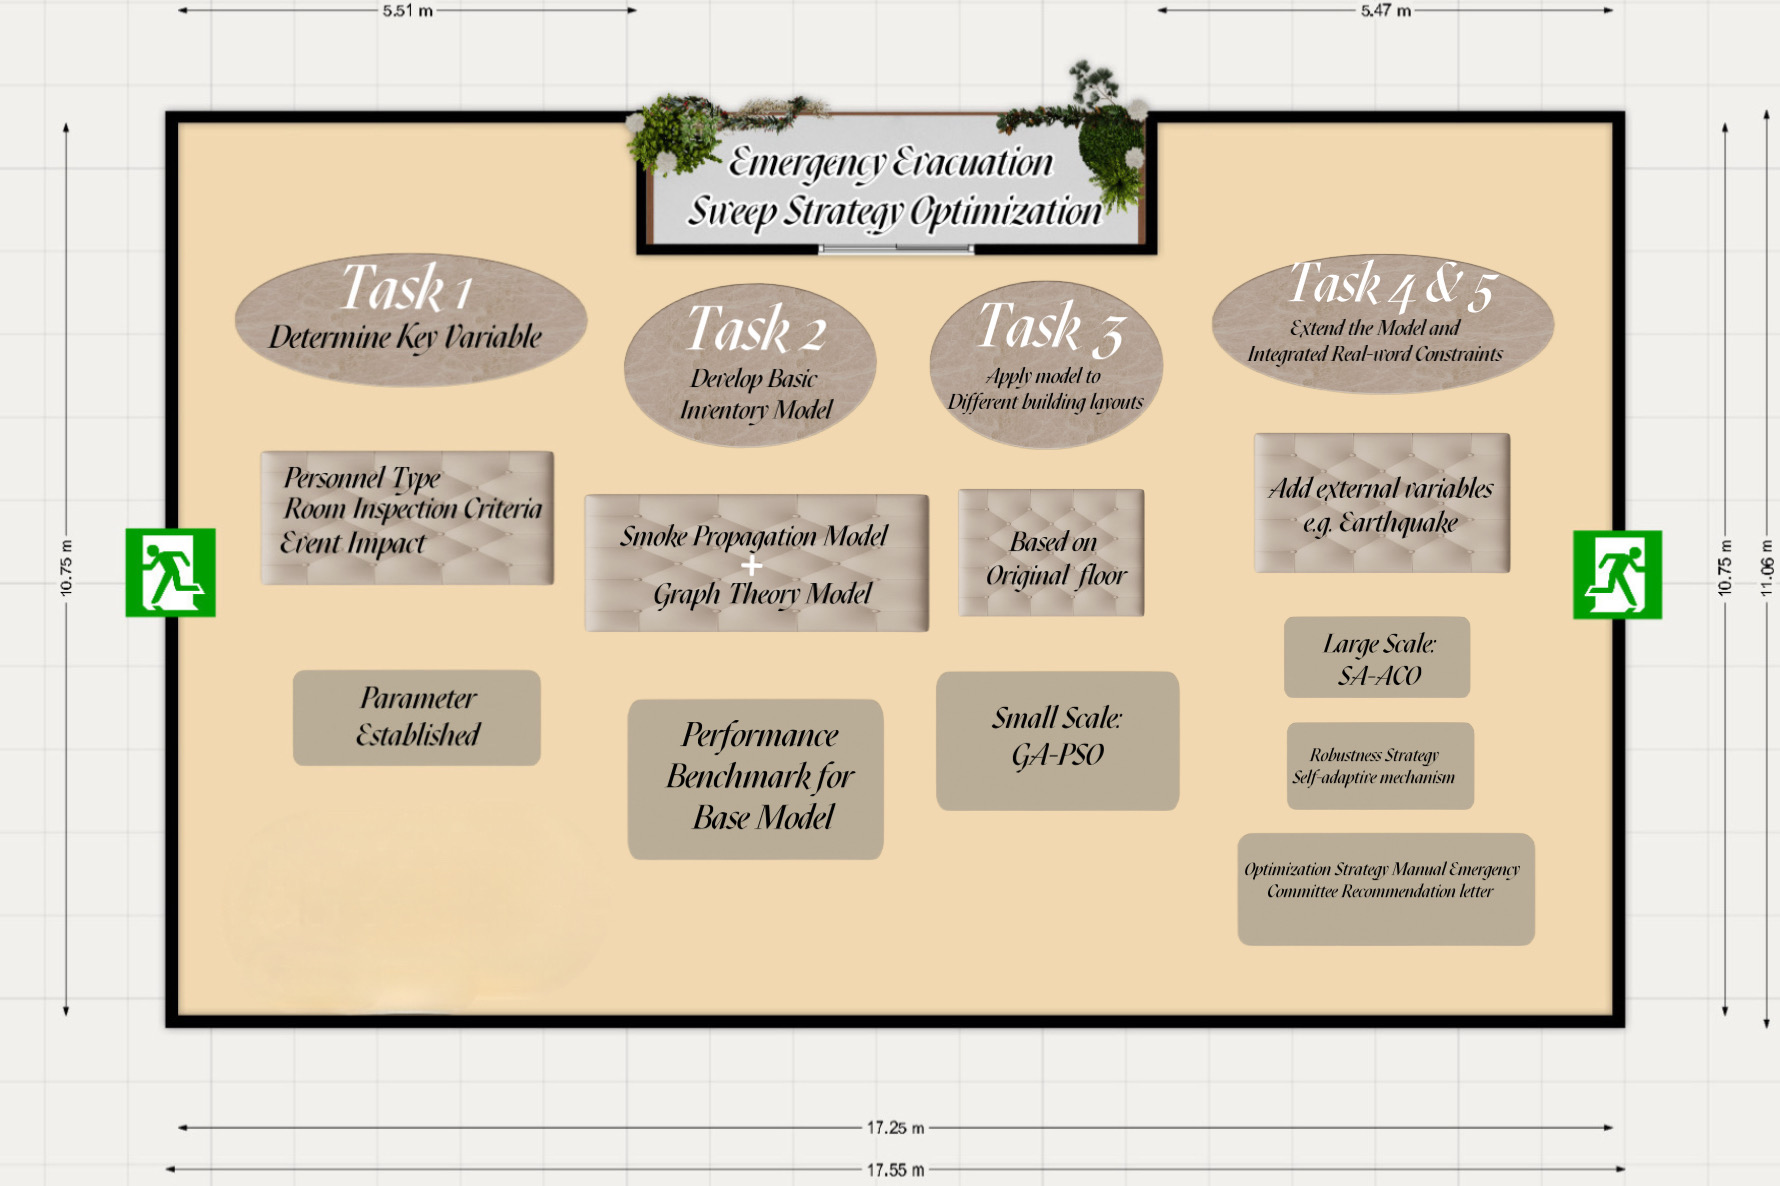
\includegraphics[width=.99\textwidth]{ourwork.png} 
	\caption{The flow chart of our work} 
	\label{ourwork} % 图片标签
\end{figure}

\vspace{-0.3cm}%设置上下的距离，可正可负，一般用于缩小图片或者表格与下方文字的较大空间，但若文字或者表格浮动到下一页，可能会导致文字重叠，慎用



%\begin{itemize}
%	\setlength{\parsep}{0ex} %段落间距
%	\setlength{\topsep}{2ex} %列表到上下文的垂直距离
%	\setlength{\itemsep}{1ex} %条目间距 这三句的效果就是各条内部的文字贴在一起，条与条之间分得很开，否则就是每条内部行间距比条目之间的间距都大
%	
%	\item Build a ...
%	
%	\item Adjust ...
%	
%	\item Identify ...
%	
%	\item Select...
%	
%\end{itemize}
		\section{Assumptions and Justifications}
\vspace{-0.3cm}%在\end{table}下加一行\vspace{-1cm} 其中-1的作用是缩短与下方文字距离的 切记！必须是负数

%Considering that there are complex unknown factors in practical problems, reasonable assumptions are made to simplify the model.
%无论是什么赛题，都应该明确列出所用到假设条件并解释其合理性
%评委们会审视这些假设是不是在后续的论文里被用到

\textbf{1.Perfect Information and Training:} Assuming all responders have identical training, perfectly recall the building layout, and execute commands without error.

   \textbf{    Justification:} This isolates the optimization problem from human performance variability and communication delays, allowing us to focus on the intrinsic efficiency of the sweep strategy itself. Subsequently, by introducing parameters such as information error rate and execution fault tolerance rate, it can gradually approach the actual scenario.


\textbf{2.Stable Site Conditions:} Assuming that factors such as explosions or earthquakes that cause room collapse are not considered. After an emergency occurs, the layout structure and physical distances of the site remain unchanged.

\textbf{Justification:} Stabilizing the site condition can simplify the basic model and provide stable spatial constraints for optimization tasks such as path planning and task allocation.


\textbf{3.Reponder Safety and Capability Assurance:} This means emergency response personnel of different professional types have received professional training, are equipped with sophisticated equipment. Therefore, no casualties will occur during the search process on-site.

\textbf{Justification:} This eliminates the reduction in the number of personnel due to casualties, task interruptions, or strategy adjustments, allowing the model to focus solely on time optimization. The actual safety risks in the real scenario can be corrected in subsequent models by introducing a risk coefficient.


\textbf{4.Graph-Theoretic Abstraction of Architectural Space:} We discretize the complex architectural floor plan into a graph theory model G = (V, E), where \textbf{rooms and exits are abstracted} as nodes V, and\textbf{ times responders cost travelling between each nodes} are abstracted as edges E. This model ignores the specific shapes, areas, and physical properties of doors and windows of the rooms.

\textbf{Justification:} This process is a standard pre-step in network optimization problems. It transforms the continuous search space into a discrete mathematical structure, thereby providing a rigorous mathematical foundation for applying shortest path algorithms. This simplification enables us to focus on the core logic of path sequences and personnel allocation.

We also made some other assumptions to simplify analysis for individual sections. These assumptions will be raised where relevant.
\vspace{-0.5cm}%在\end{table}下加一行\vspace{-1cm} 其中-1的作用是缩短与下方文字距离的 切记！必须是负数
%如果有一些专有名词或者模糊概念的定义，可以加一个Definition版块。

		\section{Notations}
%Some important mathematical symbols in this paper are listed in Table \ref{notation}.
\vspace{-1cm}%在\end{table}下加一行\vspace{-1cm} 其中-1的作用是缩短与下方文字距离的 切记！必须是负数

\begin{table}[htbp]
	\begin{center}
		\caption{Notations Used in This Paper}
		\begin{tabular}{l l}%c居中，l左对齐
			\toprule[2pt]
			\multicolumn{1}{m{3cm}}{\textbf{Notations}}
			&\multicolumn{1}{m{8cm}}{
			\textbf{Descriptions(Unit)}}\\
			\midrule
			  $V$& Set of nodes abstracted from all rooms and exits (no unit) \\	
			  $D_{ij}$& The actual shortest spatial distance from node $i$ to node $j$ (m)\\
			  $T_{\text{move}}(i,j,k)$& Movement time of responder $k$ from node $i$ to node $j$ (s) \\
			  $T_{\text{check}}(i,k)$& The time taken by responder $k$ to check room $i$ (s) \\
			  $T_{\text{max}}$& Maximum time taken by all responders to complete the sweep task (s) \\
			  $F$& The fitness of a certain path planning scheme (no unit) \\
			\bottomrule[2pt]
		\end{tabular}\label{notation}		
	\end{center}
\end{table}

\vspace{-1cm}%在\end{table}下加一行\vspace{-1cm} 其中-1的作用是缩短与下方文字距离的 切记！必须是负数
%如果有一些专有名词或者模糊概念的定义，可以加一个Definition版块。

		\section{Model Preparation}
\vspace{-0.3cm}%在\end{table}下加一行\vspace{-1cm} 其中-1的作用是缩短与下方文字距离的 切记！必须是负数

In our plan, search and clearance is of vital importance, which involves a strategy carried by trained responders, moving from room to room ensure each trapped occupant position.

We need to clarify a definition all-clear criterion - a room is deemed \textbf{cleared} only after all \textbf{effective areas} (accessible spaces where people might stay, such as under desks, behind shelves, enclosed corners) have been visually or physically inspected, confirming no trapped persons or hazards exist\upcite{6}. This criterion applies to all scenarios but adjusts dynamically based on room layout like checking cribs in childcare centers or file cabinets in offices.

To address the problem of minimizing search time under information-constrained emergency conditions by optimizing the sweep and check processes of emergency personnel, this section clarifies the core elements of the model, defines key parameters, and establishes a quantitative calculation framework for \textbf{clearance time}, laying the foundation for subsequent combinatorial optimization.

Informed by emergency management practices (e.g., standardized sweep procedures in response manuals)
\upcite{7}
%这里可以引用参考资料 
and analogous optimization research, the model design is governed by five interconnected elements, each quantified by parameters or sub-models.

    \begin{itemize}
    \item \textbf{$C$ (Environmental Complexity Coefficient)} 
    \end{itemize}
    
    Environmental complexity coefficient $C$ is to quantify the obstacles caused by the physical environment of the room to the investigation, which value adjusted linearly is based on the density of spatial obstacles (such as shelf spacing and the number of furniture). It is also affected by smoke diffusion.

    
    \begin{itemize}
    \item \textbf{$L$ (Layout Complexity Coefficient)} 
    \end{itemize}
    
    In order to improve the accuracy of the model, we consider the three-dimensional room layout as a two-dimensional one, which can also enhance adaptability. Sweep complexity is significantly driven by occupant type, and $L$ quantifies this as a dimensionless coefficient. It scales from 1.0 for simple offices to 2.0 for high-complexity spaces like childcare centers or warehouses.


    \begin{itemize}
    \item \textbf{$E$ (Incident Impact Coefficient)} 
    \end{itemize}
    
    Incident impact coefficient $E$ represents the indirect impact of non-structural incidents on search operations (e.g., reduced visibility due to fire). It ranges from 1.0 (no impact, e.g., false alarm) to 1.3 (mild impact, e.g., low-concentration smoke) and is dimensionless. Incidents causing severe environmental changes are excluded from the current model. Notably, this may be a time-related coefficient.
    
    \begin{itemize}
    \item \textbf{$A$ (Effective Area)} 
    \end{itemize}
    
    $A$ represents the actual, accessible floor space requiring a sweep (excluding walls and fixed structures), measured in $\text{m}^2$. A linear relationship between sweep time and area ($A$) is assumed.
  
    \begin{itemize}
    \item \textbf{$R$ (Redundancy Coefficient)} 
    \end{itemize}
    
    The basic model does not currently involve redundancy strategies. In the expanded model, a redundancy coefficient ($R$) will be incorporated as a time multiplier. For example, $R=1.2$ indicates an additional 20\% check time.



    \begin{itemize}
    \item \textbf{$\alpha_c$ (Checking Velocity)} 
    \end{itemize}

    According to the professional type, responders can be classified into 3 types (with coefficients arranged in descending order): Trained fire captain, regular firefighter, and security guard. The parameter $\alpha_c$ reflects the checking velocity with unit $\text{m}^2/\text{s}$. In addition to the search speed of the room, the movement speed also needs to be defined. 
    
    \begin{itemize}
    \item \textbf{$\alpha_m$ (Moving Velocity)} 
    \end{itemize}

    $\alpha_m$ reflects the moving velocity with unit $\text{m/s}$. Similar to the checking speed, responders are classified into 3 types with each a different expected value of normal distribution. The moving speed is particularly influenced by visibility, which can be affected by the spread of smog; thus it can also become a function of time.

    
Assumptions have been made about Responders in the previous section. Based on a Gaussian distribution, the two types of speeds of the same type of personnel both follow a normal distribution, with their expected values denoted as \( \alpha_m \) and \( \alpha_c \), which can be adjusted. Specially, when considering the spread of smog, the checking velocity varies with time (also seen in Task 4).

We then define \textbf{the room search volume to clear}: \(Q = C \cdot L \cdot E \cdot A \cdot R\), where \(Q\) has the units of \(\text{m}^2\). So we can obtain the expression for check time \(T_{\text{check}} = Q/\alpha_c\), where \(T_{\text{check}}\) has the dimension of \(\text{s}\).
    
    
    As listed in Table \ref{notation}, \(D_{ij}\) represents \textbf{the actual shortest spatial distance} from room \(i\) to room \(j\). For buildings with complex structures, we need to draw a mask based on the architecture's layout and use \textbf{A* algorithm} to find the shortest path distance between two rooms while bypassing obstacles. 
    
    But more commonly, in simple scenarios, the Euclidean Distance and Manhattan Distance are used with the formulas: \(D_{euclidean} = \sqrt{(x_1 - x_2)^2 + (y_1 - y_2)^2}\) and \(D_{manhattan} = |x_1 - x_2| + |y_1 - y_2|\). Then we can obtain the time a responder needs to move from room \( i \) to room \( j \) \( T_{\text{move}} = D/\alpha_m\). Take the layout in Figure\ref{fig:layoutpre} for an example, doors of the rooms are marked with red stars. For environment with cubic obstacles, we can also use the Manhattan distance to calculate.

\begin{figure}[htbp]  % h表示此处，t表示页顶，b表示页底，p表示独立一页，控制浮动体位置
    \centering
    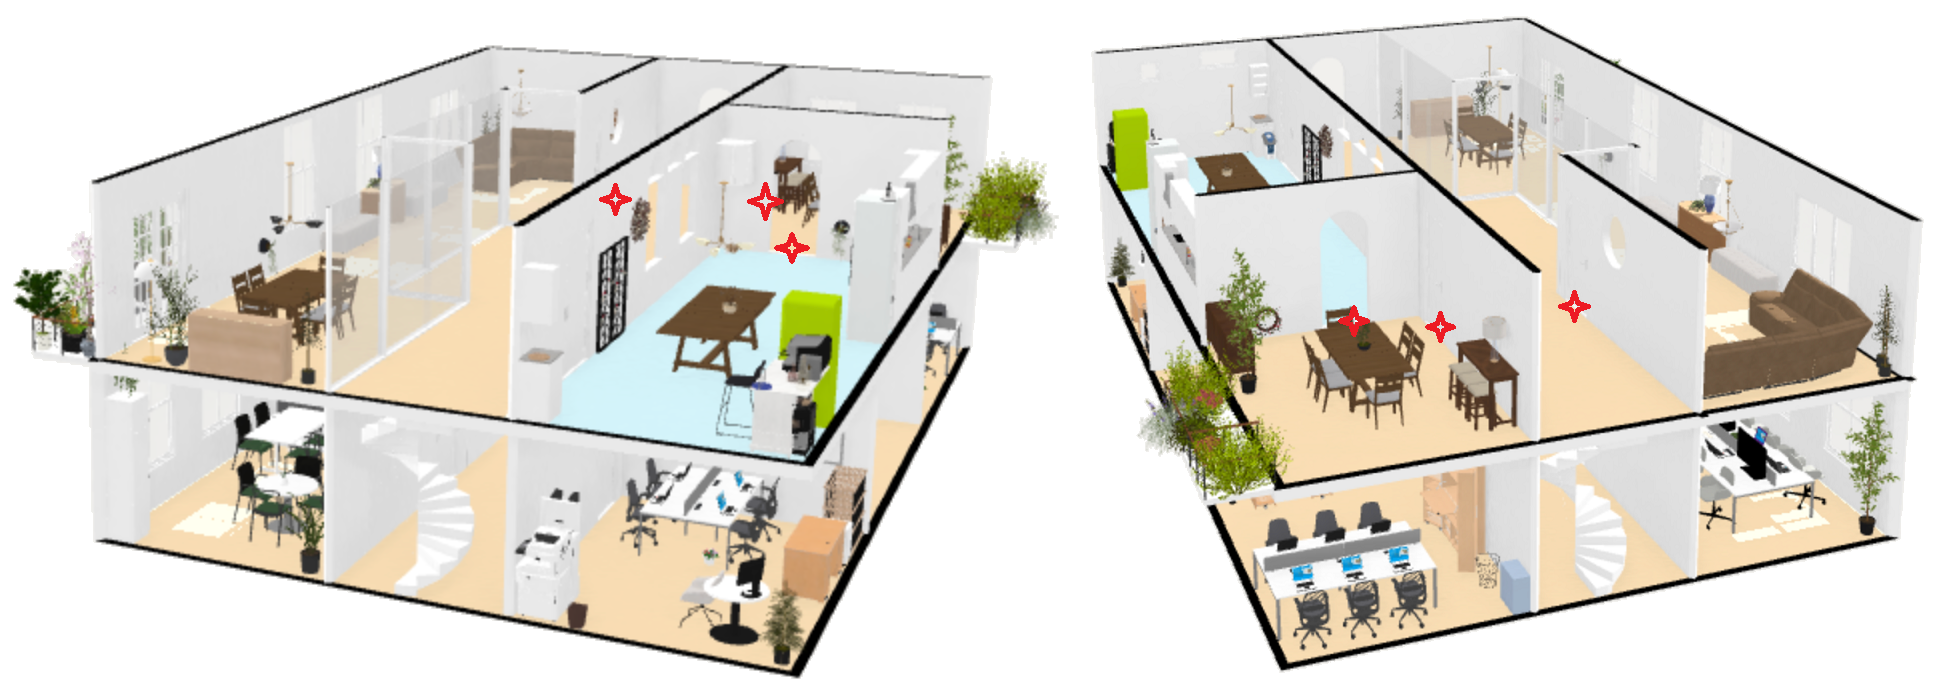
\includegraphics[width=0.85\linewidth]{layoutpre.png}
    \caption{Layout of a Two-Story Daycare Center}
    \label{fig:layoutpre}
\end{figure}

Finally, the time for a firefighter to travel from room \( i \) to room \( j \) plus the search time is calculated as \(T_{\text{sweep}} = T_{\text{check}} + T_{\text{move}} \). This quantifies the clearance time for a single room by integrating room characteristics, personnel capabilities, and environmental factors, providing fundamental input for subsequent combinatorial optimization of multi-room and multi-personnel scenarios, such as path allocation and task scheduling.

\vspace{-0.1cm}%在\end{table}下加一行\vspace{-1cm} 其中-1的作用是缩短与下方文字距离的 切记！必须是负数

		\section{Graph-Metaheuristic Optimization Model for Responder Sweep Scheduling}

\vspace{-0.2cm}%在\end{table}下加一行\vspace{-1cm} 其中-1的作用是缩短与下方文字距离的 切记！必须是负数

\subsection{The Abstraction of Graph Theory}

How to assign firefighters and determine the order in which firefighters travel through room to minimize the total time consumed? We attempt to abstract the objects of this problem using \textbf{graph theory}.


We consider the object of study as a connected graph, where the rooms and exits on the map form the vertex set \( V \), and edges connect these vertices. The problem requirement can also be abstracted as: assign the vertices in the vertex set \( V \) to \( m \) firefighters, allowing them to start from safe exit vertices, traverse the assigned vertices in a certain order, and then leave from some safe exit vertices. The edge weight of the graph is the time \( T_{\text{sweep}} \) for the responder to start from one point and finish checking and clearing the next point.






Based on the graph theory "node-edge-weight" abstraction system and multi-objective optimization algorithms, the model automatically completes three core tasks:


1. Room assignment of the responders

2. Path planning of each responders

3. Fitness scoring of each combined scheme


\begin{itemize}
    \item Fitness scoring of each strategy
\end{itemize}


The evaluation metric for each combined scheme is called \textbf{fitness}.
To unify dimensions, exponential decay normalization is adopted. Let the normalized fitness value be $\hat{F}$ and the maximum total time be $T_{max} = \max(T_{\text{total}})$. The normalization formula is: \(
\hat{F} = 1 - e^{-k \cdot \max(T_{\text{total}})}\), where $k > 0$: an adjustment parameter that controls the convergence speed of fitness as $\max(T_{\text{total}})$ increases.

Given the median of the maximum total time as $\max(T_{\text{total}})$, set the fitness at this point to 0.5. Solving for $k$ gives:\(k = \ln 2/\max(T_{\text{total}})\).

\begin{figure}[htbp]
    \centering
    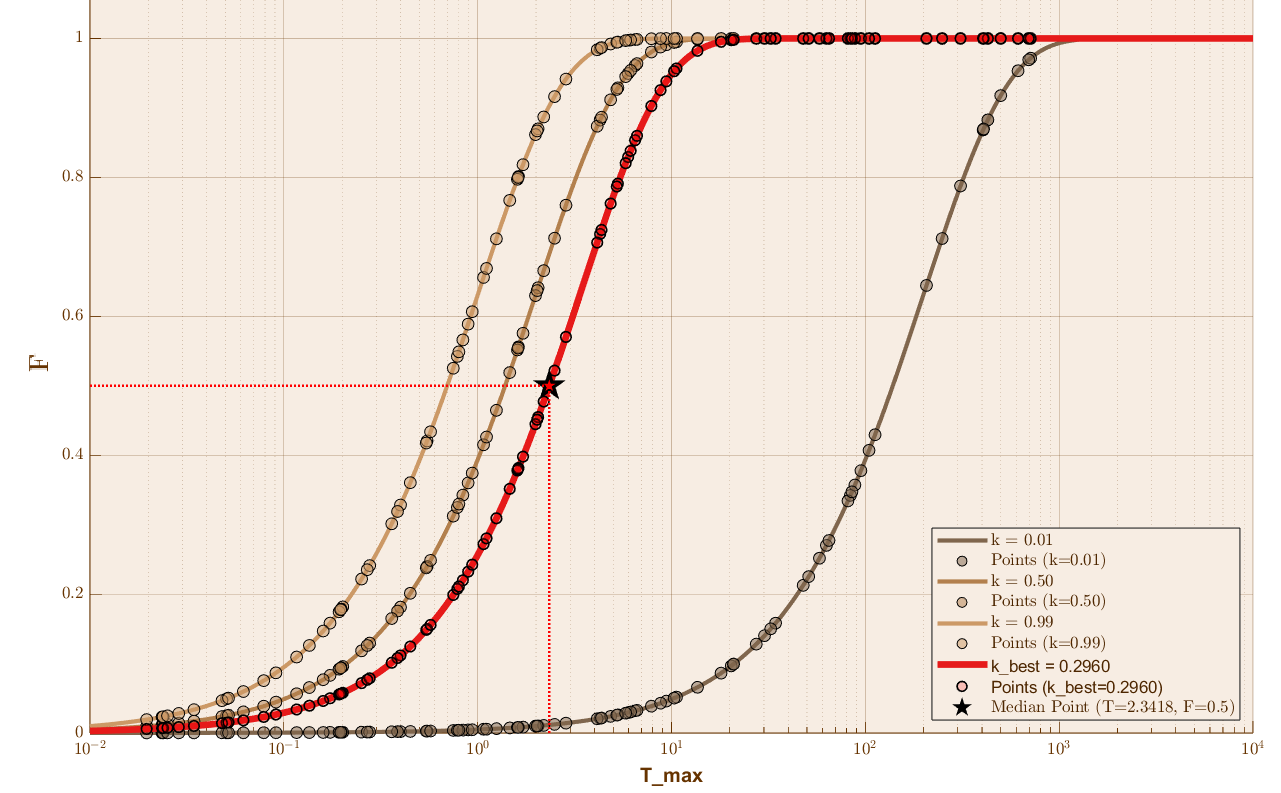
\includegraphics[width=0.85\linewidth]{fig/fitness.png}
    \caption{Best-k-Normalization of Randomly Generated $T_{max}$}
    \label{fig:fitness}
\end{figure}
\vspace{-0.3cm}
This formula maps the maximum total time to the interval [0,1] via the saturation of the exponential function, making it suitable as a fitness function in optimization models and balancing the impact of maximum time at different scales on the optimization objective.


\subsection{The Algorithm of Metaheuristic Optimization }

Given the allocation and traversal order, the total time is determined by the slowest firefighter (aiming to minimize this time).For NP-hard problem like this, brute force enumeration is costly, and \textbf{metaheuristic algorithms} can efficiently find approximate optimal solutions.

However, before that, we need to precisely express the allocation and permutation of a scheme. Hence, encoding:  

For $m$ firefighters $M_1$ to $M_m$, $n$ rooms $N_1$ to $N_n$, the encoding is $[N_1, N_2, N_3, \ldots, N_n \mid x_1, x_2, x_3, \ldots, x_m]$ (where $\sum x_i = n$). The first segment of the encoding $N_1, N_2, N_3, \ldots, N_n$ represents dividing these points (rooms) into $m$ groups, with the number of rooms in each group being $x_1, x_2, x_3, \ldots, x_m$ respectively. Note that the order of N only indicates the allocation of rooms, not the traversal order for each firefighter. For example, if a firefighter is assigned rooms $N_1$ and $N_2$, the order could be $N_1 \to N_2$ or $N_2 \to N_1$.  

Additionally, we do not mention entrances and exits in the encoding -we allow firefighters to enter from the exit closest to the first room and leave from the exit closest to the last room.  


\subsection*{Algorithm 1: Simulated Annealing Nested with Ant Colony Optimization}

To minimize time consumption, we recognize that equal allocation is a relatively optimal initial solution before traversal. Therefore, we adopt the following initial allocation: ensure that the number of rooms assigned to the firefighter with the fewest rooms is at most one less than the number assigned to the firefighter with the most rooms. That is:  

\(
x_{\text{max}} - x_{\text{min}} \leq 1, \quad \text{for } N \in \mathbb{Z}^+
\)

Now, consider using Ant Colony Optimization to determine how to order the firefighters' routes to minimize the total time consumption. 

Imagine that before setting out, firefighters release many ants to explore the optimal route. Ants leave pheromones on the paths they traverse. We assume that an equal amount of pheromone $Q$ is deposited on each path from one room to another. Thus, the increase in pheromone concentration $\Delta \tau$ on the path from point $n_i$ to $n_j$ due to an ant passing is:  

\(
\Delta \tau = \frac{Q}{L_k}
\)

Pheromones will evaporate so we set a parameter $\rho$ to represent the evaporation rate, which is a value in the interval [0,1]. Thus, the pheromone concentration on the path from $n_i$ to $n_j$ at time $t+1$ is:  

\[
\tau_{ij}(t+1) =  \rho \cdot \tau_{ij}(t) + \Delta \tau
\]

where $\tau_{ij}(t)$ is the pheromone concentration on the path at time $t$.  

Ants consider paths with higher pheromone concentrations to explore optimal solutions, as this indicates that more individuals have chosen this path. Thus:  

\[
p_{ij}^k  \propto \frac{(\tau_{ij}^\alpha)}{\sum_ (\tau_{iz}^\alpha)}
\]


where $P_{ij}$ is the probability that an ant at $n_i$ decides to go to $n_j$ next, and $\alpha$ is a parameter describing how much pheromone influences $P$. The denominator is the sum of pheromone concentrations over all possible paths.  

Simultaneously, ants also consider the distance between rooms. The greater the distance $D$ is, the less an ant will want to go there. Therefore, we define the inverse of distance as $\eta$. Similarly, $P_{ik}$ should be proportional to $\eta_{ij}^\beta$ divided by the sum of $\eta_i^\beta$, where $\beta$ describes the weight of the distance factor's influence on $P$. That is: \(P_{ij} \propto \eta_{ij}^\beta/\sum \eta_i^\beta\)

Thus, we have:  
\[
p_{ij}^k  =\frac{(\tau_{ij}^\alpha)(\eta_{ij}^\beta)}{\sum_ (\tau_{iz}^\alpha)(\eta_{iz}^\beta)}
\]

After multiple repetitions, the ants will converge on one path, which is the approximate optimal route. The firefighters can then follow this route. We calculate the time consumption for each firefighter and take the maximum as the total time consumption of this scheme.  

The problem now is how to update to a new allocation. We adopt the simulated annealing model. The general idea is: continuously attempt to find an allocation scheme that minimizes the total time consumption of the scheme; when the total time of a newly attempted scheme is less than the original total time, we always accept the new allocation; but if the new scheme's total time is greater, we accept it with a certain probability. This can be explained as follows---imagine the following graph, where the vertical axis represents the total time, and each point on the horizontal axis represents a new scheme. The goal is to find the minimum value of the entire function. Note that during the attempt, the entire function's shape is unknown; only the value of the next point is visible. When the next value is larger, to avoid being trapped in a local optimum and unable to cross the peak A to reach a smaller value B, we need to weigh whether to accept it.  

This trade-off is represented by the probability $P(\text{accept})$. When $P(\text{accept}) > 0.5$, we accept this risky change. According to previous research in thermodynamics, this probability is a natural exponential:  \(P(\text{accept}) = e^{-\frac{\Delta T}{T}}\), where $T$ is the total time of the original scheme, $T'$ is the total time of the newly attempted scheme, and $\Delta T$ is the change in total time---equal to $T' - T$.  

The model will continuously attempt until it oscillates around a value, which can be considered a relatively optimal solution.  

The only remaining problem is how to attempt. We should not spend too much effort on this as it should be random. Therefore, we define that each attempt can choose one of the following two operations: 1. Randomly exchange one room between two firefighters. 2. Transfer one room from one firefighter to another. The selection of firefighters and rooms is also random.  

\subsection*{Algorithm 2: Genetic Algorithm Fused with Particle Swarm Optimization}

If we consider the order of N in the encoding as the traversal order of the firefighters, this means that one segment of the encoding contains all the information of the scheme (i.e., allocation and order). We can directly use a calculation similar to Algorithm 1 to compute the total time consumption of an encoded scheme.  

The focus shifts to how to perform iterations: First, because it can be imagined that without the ant colony optimization for the optimal solution of each allocation, the iteration volume we obtain will be larger---to alleviate this computational and storage pressure, we fix the sample size of results for each iteration to $n$, and we only iterate on this group. Second, if the iteration of the group involves all encodings, it may lead to the loss or degradation of high-quality encodings. Therefore, before each iteration, we sort the encodings in the group from smallest to largest based on time consumption and retain the top 10\% of encodings to directly skip the iteration and enter the next group. It should be noted that this does not preserve stubborn encodings because even if retained into the next group, less excellent encodings will lose their top 10\% position in the next group's sorting and fall into iteration.  

After overcoming all difficulties, the only problem left is how to iterate. Imagine each encoding as a DNA double helix (one helix is the N sequence, the other is the x sequence). We mimic the crossover and mutation of DNA for iteration:  

Crossover between two DNAs involves selecting the same segment of encoding from the father's and mother's N sequences for exchange, while the x sequence remains unchanged, retaining the father's result as the offspring. Note that the N sequence can only crossover with the N sequence, and the x sequence can only crossover with the x sequence, exhibiting isolation. Crossover has directionality; the offspring will move in the direction of the mother based on the father.  

Mutation targets a single DNA, meaning extracting a segment from the N sequence and x sequence respectively, shuffling it, and then putting it back. Mutation is random because the probability of the shuffled encoding's score increasing or decreasing is equal.  

Then, who should be chosen as the mother? We refer to the particle swarm model---imagine each DNA is a particle. Many DNAs have already crossed with each other to form a large genetic tree. Each particle has a score at its current position, and the particle will move to try to find the point with the smallest score. The movement speed is: First, there is its own inertial velocity, which is random, manifested as DNA mutation. Second, it will move towards the point with the lowest score in its own historical path, manifested as the DNA crossing over with the one with the lowest score in its direct parental line. Third, not only one particle is moving and scouting; it will also move towards the point with the lowest score found by all particles' scouting, manifested as crossing over with the DNA with the lowest score in the entire lineage.  

In our model, we can understand it as follows: first, perform multiple random crosses on the initially generated initial group to obtain a genetic tree (note that pairwise crossing should not be done as this would cause the sample size to explode, resulting in more than $n$ encodings). Then, we randomly extract $a\%$ from the DNAs entering the iteration for mutation, $b\%$ for crossover with their best parent respectively, and $1-a\%-b\%$ for crossover with the historically best DNA.  






\subsection{Application in Single-story Office Building}
In the first scenario, we mainly focus on the single-story planar building. As shown in Fig \ref{fig:building_distance}(a), it is a floor of an office building with six offices, which has a layout measuring 17 meters in length by 11 meters in width.  We abstracted the doors of the six offices and the two exits into 8 nodes.

% 插入两张图，左右排布
\begin{figure}[htbp]  % h表示此处，t表示页顶，b表示页底，p表示独立一页，控制浮动体位置
	\centering  % 图表居中对齐
	\subfigure[Layout]{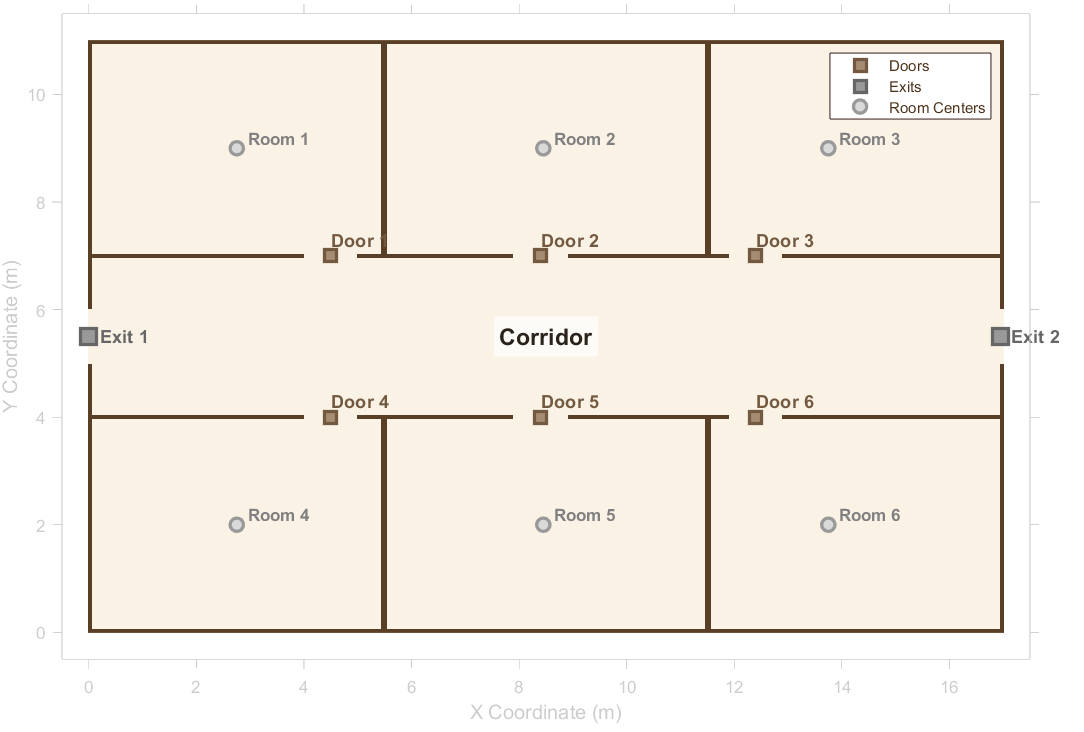
\includegraphics[width=.47\textwidth]{fig/layout1.png} % 注意图片名称或路径中不要有空格，否则会出错
	 }  % 补充右括号，修正子图标签格式
	\subfigure[Distance]{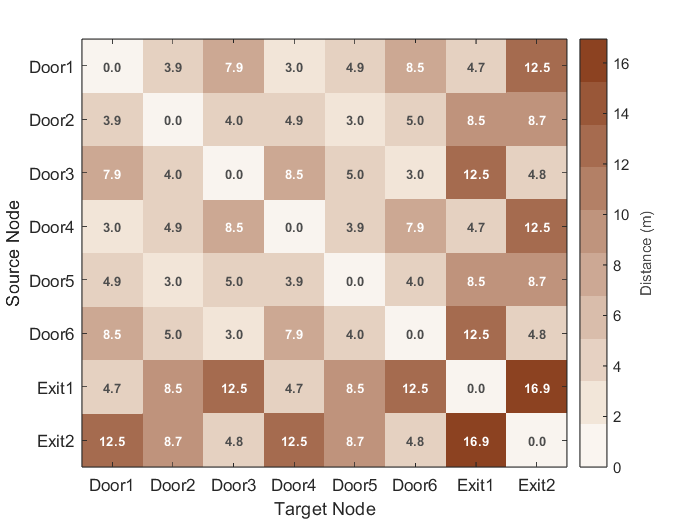
\includegraphics[width=.43\textwidth]{fig/Distance1.png} % 注意图片名称或路径中不要有空格
	 }  % 补充右括号，修正子图标签格式
	\caption{Building Layout and Inter-Room Distance Diagram}
	\label{fig:building_distance}  % 为整个图表添加主标签，便于后续引用
\end{figure}

\vspace{-0.5cm}%在\end{table}下加一行\vspace{-1cm} 其中-1的作用是缩短与下方文字距离的 切记！必须是负数

Then, the Euclidean distance is used to calculate the distance of each entrance (Fig \ref{fig:building_distance}(b)).  % 补充括号，规范图片引用格式
This value is substituted into the formula from the previous step of the model preparation process  % 修正"Mi surname"为"model"，应为笔误
and used to calculate $T_{\text{moving}}$. 

We have already determined the effective area of each office room $A=23\ \text{m}^2$. In simple offices, $L=1.0$, $C=1.0$, $E=1.0$ and $R=1.0$. So $Q=23\ \text{m}^2$.  % 单位前添加空格，补充括号使注释更清晰
With $\alpha_c \approx 0.4\ \text{m}^2/\text{s}$ 
(which matches a fire captain's speed), $T_{\text{check}} \approx 60\ \text{s}$.  

% 插入两张图，左右排布
\begin{figure}[htbp]  % h表示此处，t表示页顶，b表示页底，p表示独立一页，控制浮动体位置
	\centering  % 图表居中对齐
	\subfigure[ Simulated Annealing Algorithm]{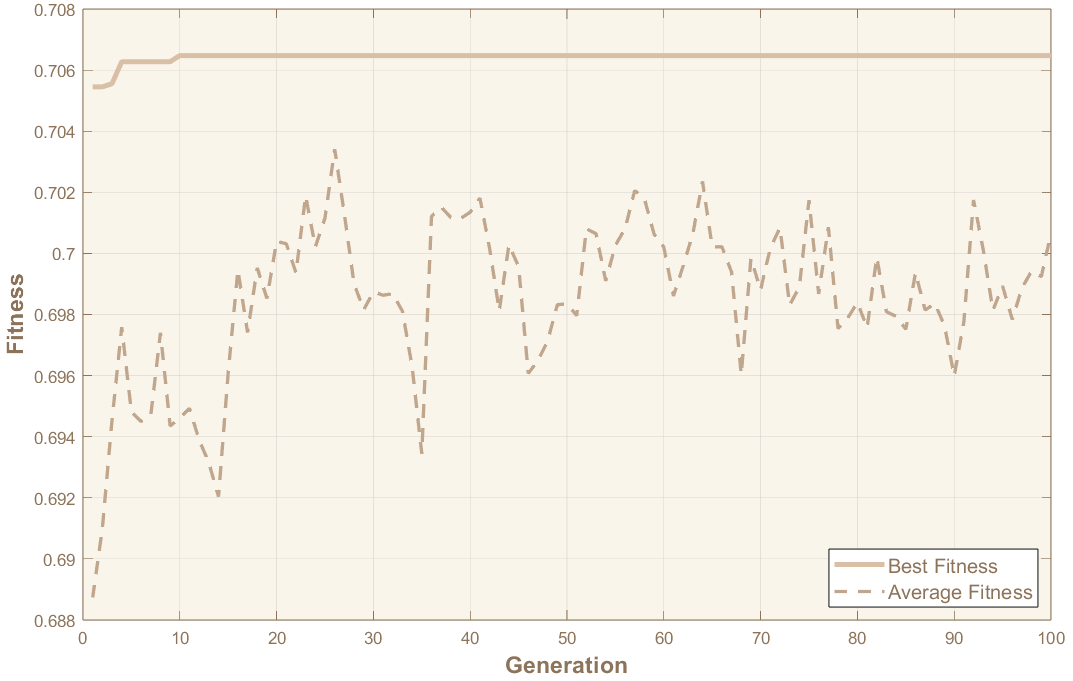
\includegraphics[width=.44\textwidth]{fig/Genetic Algorithm Fitness Evolution.png} % 注意图片名称或路径中不要有空格，否则会出错
	  \label{GA1}  % 补充右括号，修正子图标签格式
      }
	\subfigure[ Genetic Algorithm]{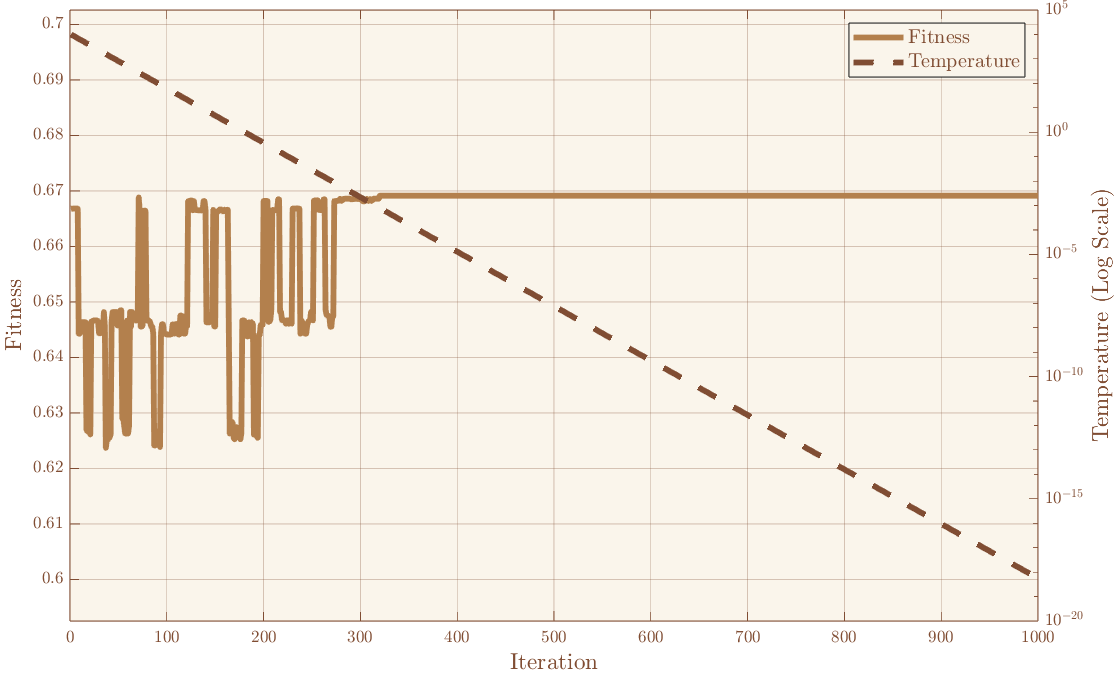
\includegraphics[width=.46\textwidth]{fig/SA1.png} % 注意图片名称或路径中不要有空格
	  \label{SA1}  % 补充右括号，修正子图标签格式
      }
	\caption{Curves of Algorithm Parameters vs. Iteration Number}
	\label{Algorithm Parameters}  % 为整个图表添加主标签，便于后续引用
\end{figure}
\vspace{-0.5cm}%在\end{table}下加一行\vspace{-1cm} 其中-1的作用是缩短与下方文字距离的 切记！必须是负数

Then, both GA and SA algorithm were applied for calculation. Figure \ref{Algorithm Parameters} shows the fitness evolution with iteration. In subfigure (a), the "Best Fitness" line rises steadily and stabilizes, while the "Average Fitness" line synchronously approaches it, verifying the algorithm’s ability to converge to the global optimal solution and avoid local optima. While in subfigure (b), the fitness curve gradually converges and the temperature curve decreases exponentially, reflecting the balance of the algorithm \textbf{between exploration and exploitation}.


The optimal fitness we obtained is 0.7063, corresponding to the paths: 

Firefighter 1 starts from Exit 1 → Door 4 → Door 5 → Door 6 → Exit 2; 

Firefighter 2 starts from Exit 2 → Door 3 → Door 2 → Door 1 → Exit 1 (as shown in Figrue \ref{path197.4s}(a)) % 去除多余空格，规范连接符使用

The time taken by each firefighter in this path was 197.4 seconds, and the optimal time was also \textbf{197.4 seconds.} 

% 插入两张图，左右排布
\begin{figure}[htbp]  % h表示此处，t表示页顶，b表示页底，p表示独立一页，控制浮动体位置
	\centering  % 图表居中对齐
	\subfigure[Best Scheme 197.4s]{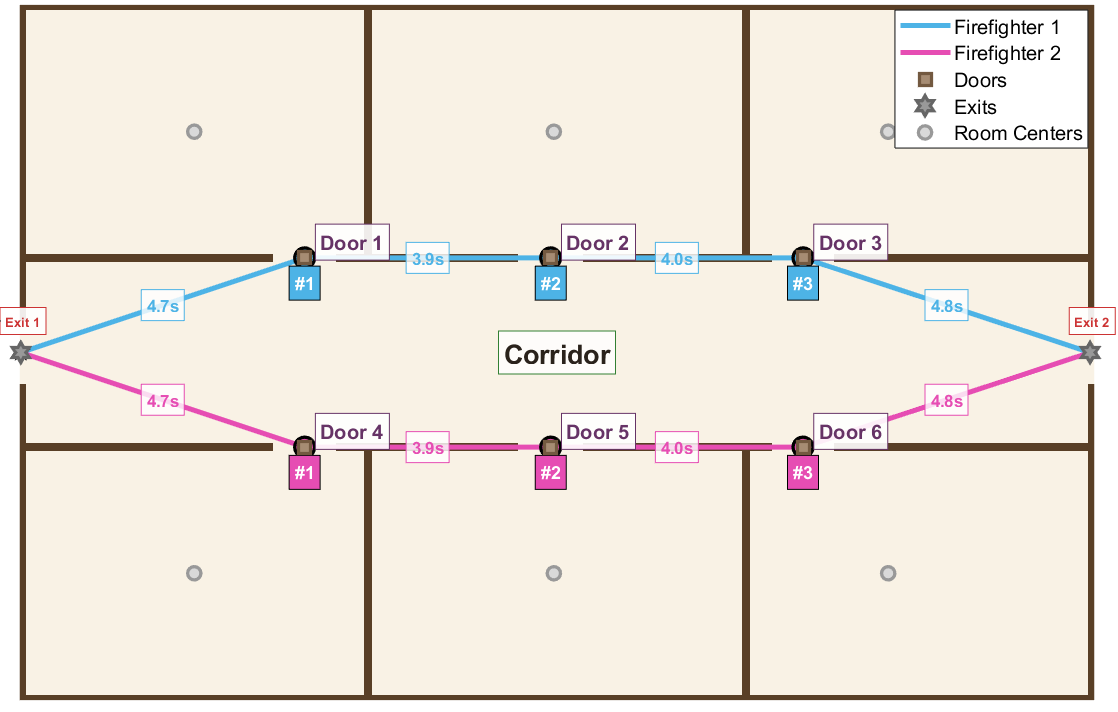
\includegraphics[width=.43\textwidth]{fig/bestpath197.4s.png} % 注意图片名称或路径中不要有空格，否则会出错
      }
	\subfigure[Second Best Scheme 198.6s]{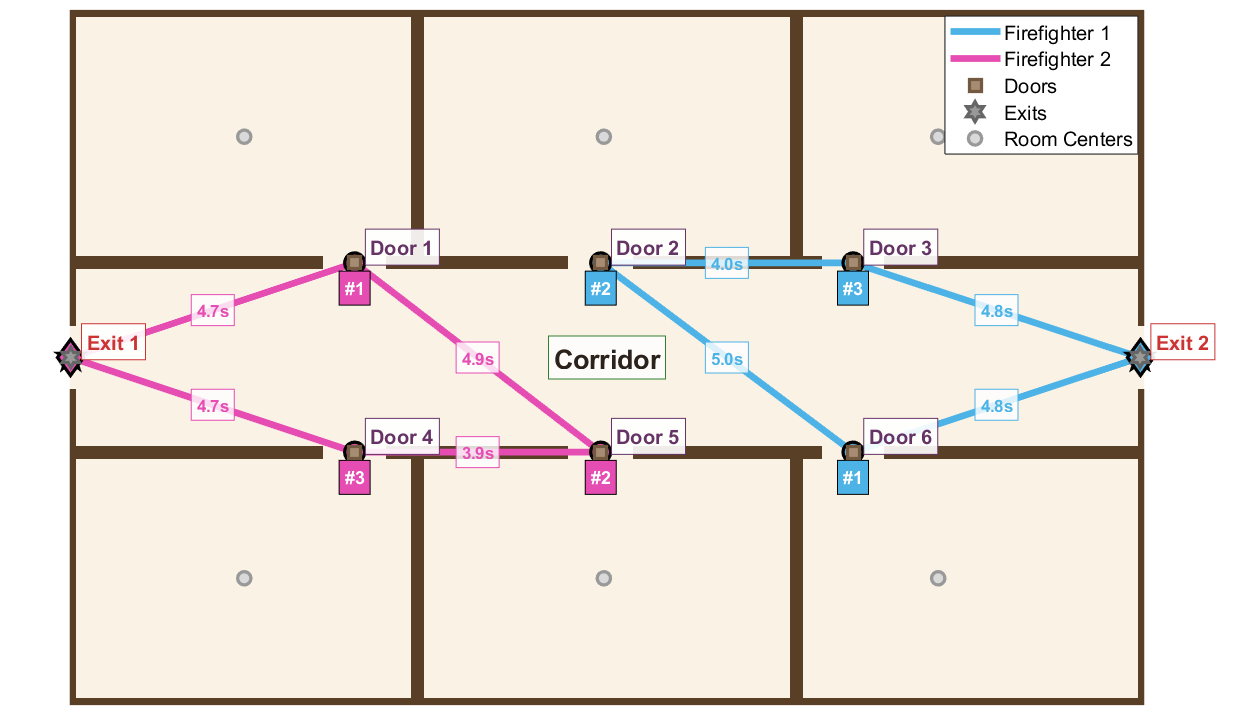
\includegraphics[width=.47\textwidth]{fig/path198.6s.png} % 注意图片名称或路径中不要有空格
      }
	\caption{Scheme for One-Story Office Building}
	\label{path197.4s}  % 为整个图表添加主标签，便于后续引用
\end{figure}
\vspace{-0.5cm}%在\end{table}下加一行\vspace{-1cm} 其中-1的作用是缩短与下方文字距离的 切记！必须是负数



For another scheme, as shown in Figure \ref{path197.4s}(b), the time consumed is almost the same, but it can ensure that the moving path of firefighters covers a smaller area, which is convenient for emergency responders to familiarize themselves with the site and carry out rescue when necessary.

When there is smoke in the fire scene, the value of the Incident Impact Coefficient (i.e., \( E \)) changes, and both the checking speed \( \alpha_c \) and moving speed \( \alpha_m \) of firefighters will decrease accordingly. We assume that the smoke concentration has an equal impact in all rooms and on the paths, and keep other parameters unchanged. Taking \( E = 2 \), \( \alpha_c \) is reduced to 10\% of its original value, and \( \alpha_m \) is reduced to three-quarters of its original value. This makes the \( T_{\text{check}} \) of each room 80s. After the algorithm runs, the optimized best path remains completely unchanged, but the maximum time consumed becomes 257.4s.

		\section{Multi-Scenario Implementation of GMO Model Based on Efficiency Evaluation}
% 两个标题均可，"Multi-Scenario Implementation..."更侧重模型的实际应用过程，"Demonstration of the Model's Applicability Across Multiple Scenarios"更强调验证模型的普适性，根据上下文选择前者更合适


\vspace{-0.5cm}%在\end{table}下加一行\vspace{-1cm} 其中-1的作用是缩短与下方文字距离的 切记！必须是负数

\subsection{Implementation to A Two-story Nursery}

For multi-floor scenarios, we maintain \( \alpha_c \approx 0.4 \, \text{m}^2/\text{s} \) and use the following settings:
- Strongly connected component: Each single floor forms a strongly connected component
- Inter-floor connection: Staircases link multiple floors into a large connected component
- Inter-floor edge length: Calculated as "current floor staircase → target floor staircase → target room"


% 插入两张图，左右排布
\begin{figure}[htbp]  % h表示此处，t表示页顶，b表示页底，p表示独立一页，控制浮动体位置
	\centering  % 图表居中对齐
	\subfigure[First Floor]{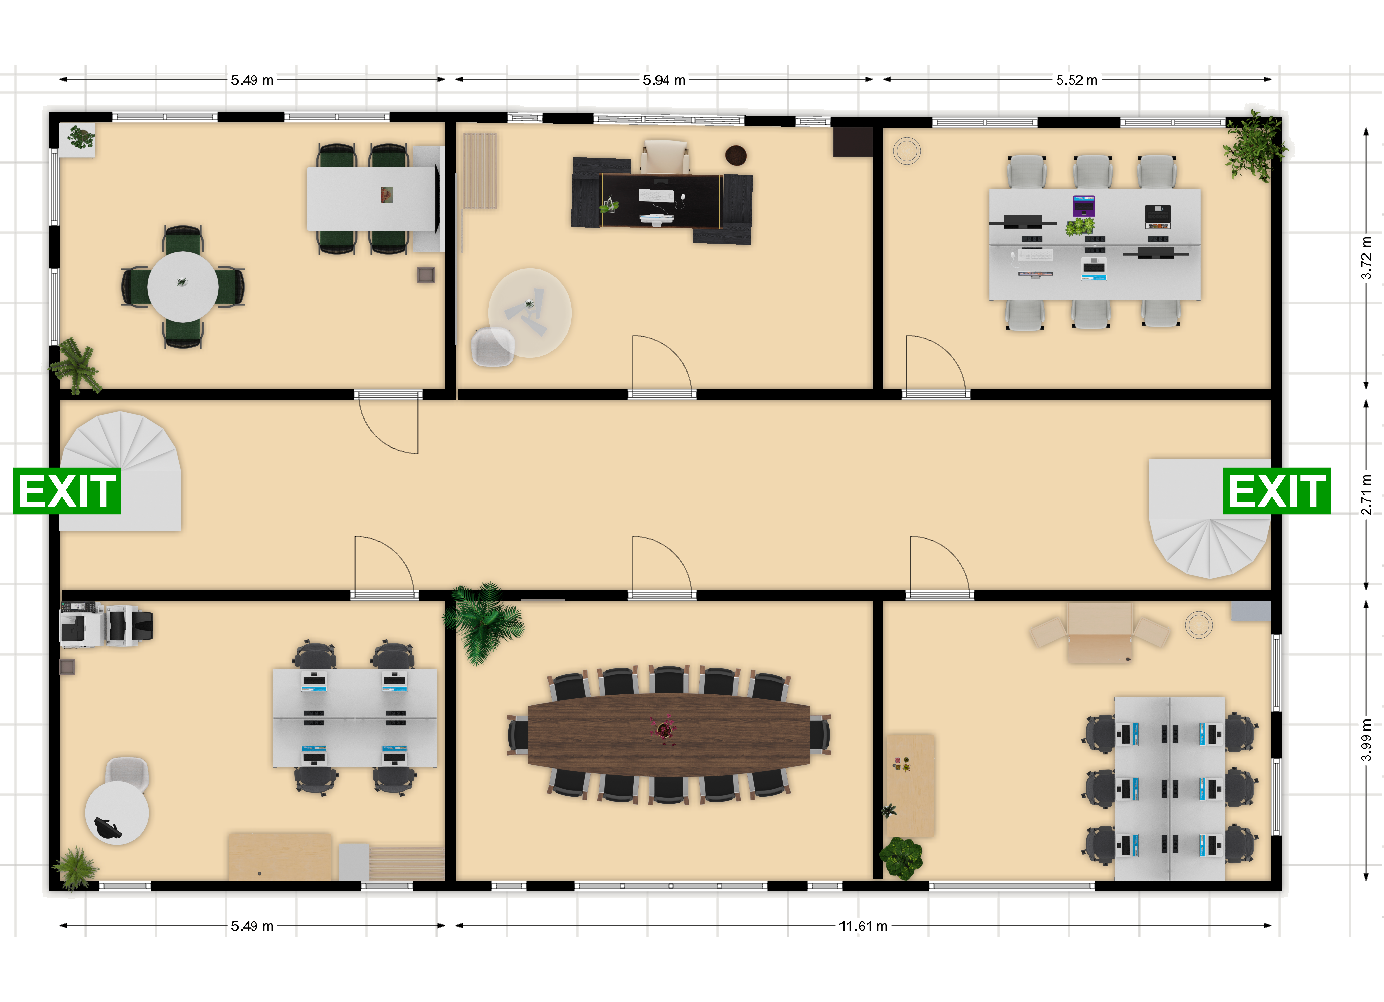
\includegraphics[width=.45\textwidth]{fig/layout21.png} % 注意图片名称或路径中不要有空格，否则会出错
      }
	\subfigure[Second Floor]{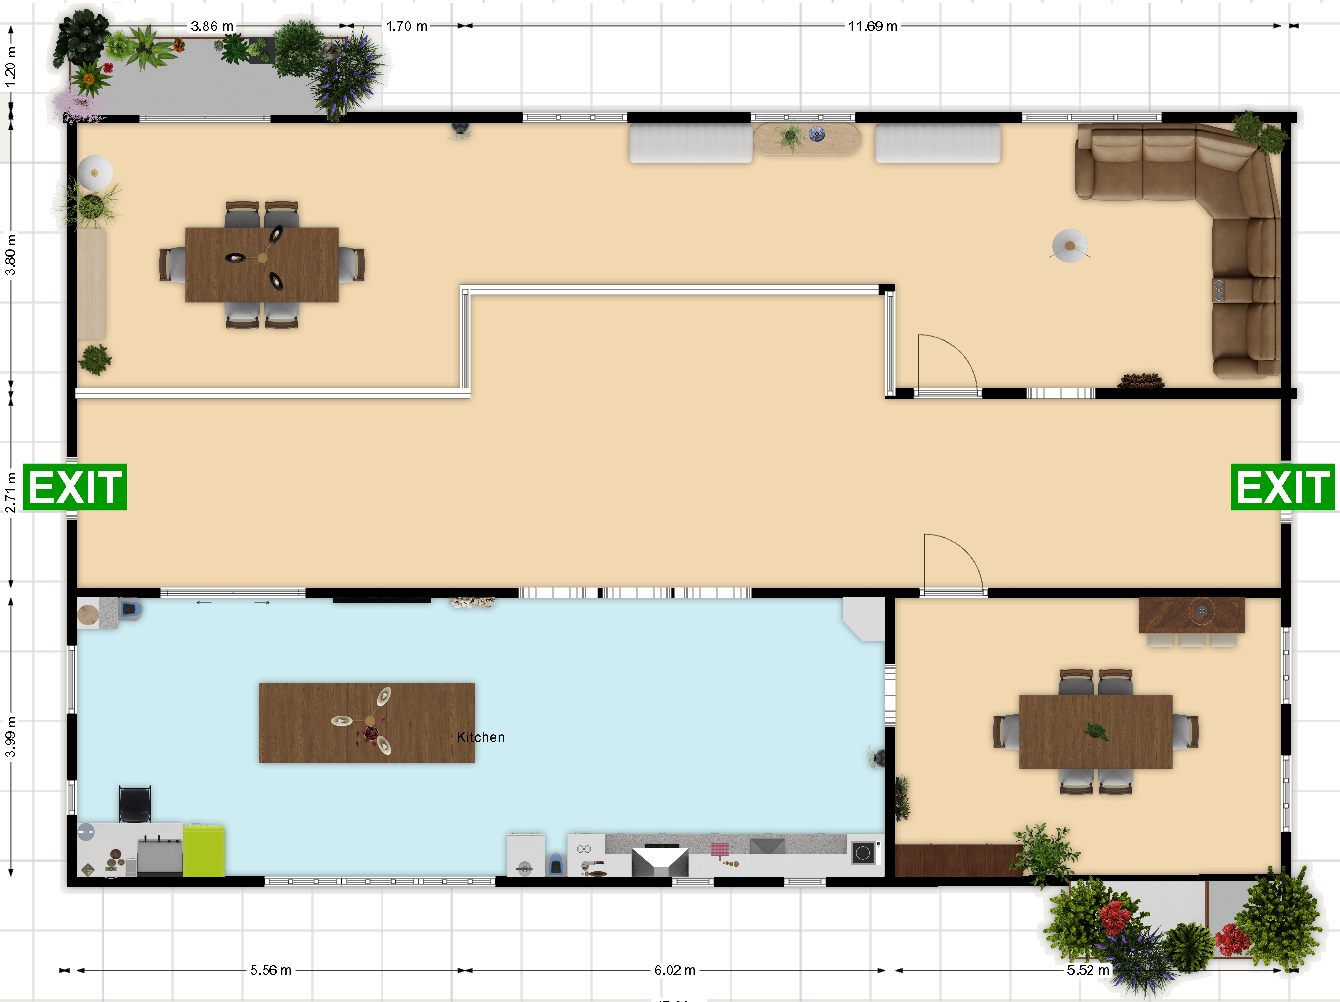
\includegraphics[width=.45\textwidth]{fig/layout22.png} % 注意图片名称或路径中不要有空格
      }
	\caption{Scheme for One-Story Office Building}
	\label{layout2}  % 为整个图表添加主标签，便于后续引用
\end{figure}
\vspace{-0.5cm}%在\end{table}下加一行\vspace{-1cm} 其中-1的作用是缩短与下方文字距离的 切记！必须是负数

The two-story nursery comprises a first-floor activity area and a second-floor rest area, connected by two spiral staircases. A corridor runs through the middle; there are two safety exits on both sides of the first floor, and spiral staircases on both sides of the second floor leading down to the first floor.

As shown in the floor plan (Figure \ref{layout2}) and the 3D diagram in the previous text (Figure \ref{fig:layoutpre}), we selected a two-story children's nursery to validate our model. Its first floor has 6 rooms with a layout similar to the office in the previous section, including 5 activity rooms and 1 craft room equipped with a large long table. The second floor features a kitchen with blue floor tiles, an adjacent dining area, and a large living room on the opposite side.

Table \ref{tab:room_parameters} presents our estimated search volumes ($Q$) for different rooms in this building.


\textbf{Floor Parameters}
\begin{table}[htbp]
	\begin{center}
		\caption{Room Parameters and Calculated $Q$ ($\text{m}^2$) Values}
		\begin{tabular}{c c c c c c c}
			\toprule[2pt]
			\multicolumn{1}{m{3cm}}{\textbf{Room Type}}
			&\multicolumn{1}{m{1.5cm}}{\textbf{Quantity}}
			&\multicolumn{1}{m{1.5cm}}{\textbf{ $A$ ($\text{m}^2$)}}
			&\multicolumn{1}{m{1cm}}{\textbf{ $ L$}}
			&\multicolumn{1}{m{1cm}}{\textbf{ $ C$}}
			&\multicolumn{1}{m{1cm}}{\textbf{ $ E$}}
			&\multicolumn{1}{m{2cm}}{\textbf{  $ Q$ ($\text{m}^2$)}}\\
			\midrule
			Activity Room & 5 & 30.00 & 1.2 & 1.2 & 1.3 & 61.78 \\
			Craft Room  & 1 & 73.72 & 1.4 & 1.3 & 1.5 & 248.47 \\
			Kitchen & 1 & 46.28 & 1.4 & 1.3 & 1.5 & 151.61 \\
			Dining Area & 1 & 36.91 & 1.1 & 1.2 & 1.3 & 69.67 \\
			Living Room & 1 & 45.59 & 1.0 & 1.1 & 1.2 & 36.19 \\
			\bottomrule[2pt]
		\end{tabular}\label{tab:room_parameters}		
	\end{center}
\end{table}



\begin{figure}[hbtp]
    \centering
    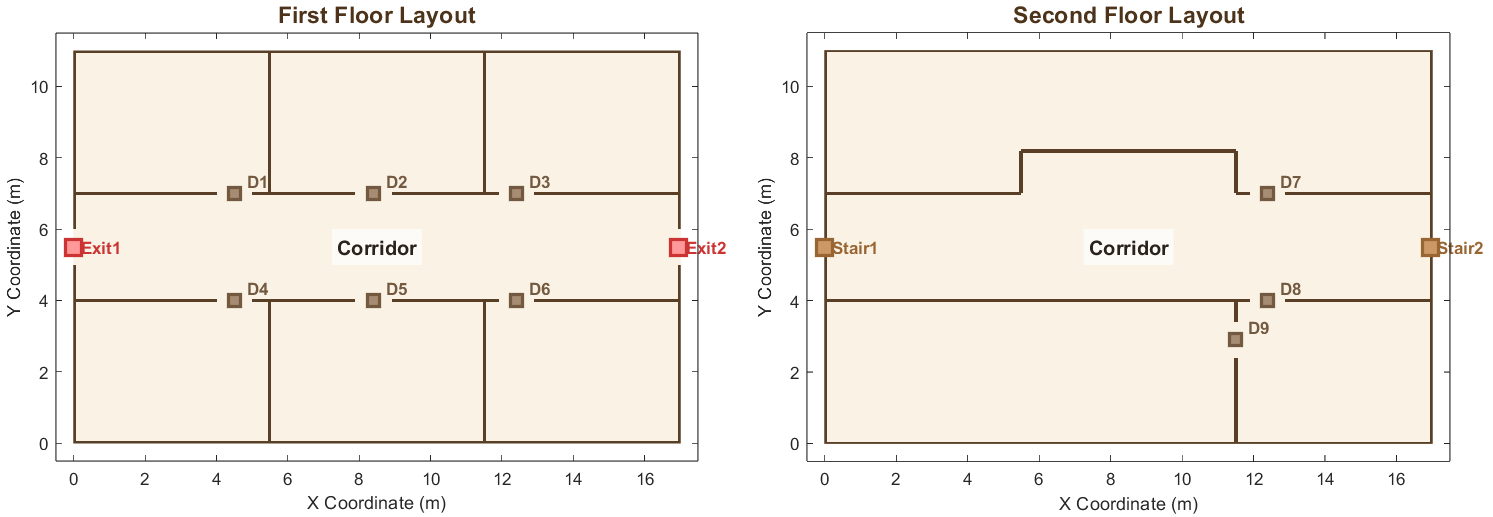
\includegraphics[width=0.75\textwidth]{fig/layout2.png} % 替换为实际图片路径
    \caption{Room Mask of the Building}
    \label{mask2}
\end{figure}

We programmed and drew room masks in the software based on the actual room layout, as shown in Figure \ref{mask}, to identify the positions of walls, safety exits, staircases, and room doors.

Then We calculated the distance for ascending and descending stairs using the inclination angle of 45° and the floor height. After abstracting room doorways as points, the Euclidean distance was used to calculate the spacing between connectable points, while the Manhattan distance was applied to points on the second floor.

Subsequently, the GA (Genetic Algorithm) and SA (Simulated Annealing) algorithms in the \textbf{GMO model} were employed to optimize the responders' paths.


However, our algorithm can actually assign any number of responders to search any number of rooms; we need to determine the optimal number of emergency responders.





\subsection{Efficiency-based Optimal Responser Quantity Evaluation}

To find the optimal number of responders, we developed a comprehensive evaluation system with a core scoring function: $S(n) = \alpha E_{\text{time}}(n) + \beta U(n) + \gamma B(n)$ . The weighting reflects that time efficiency is most critical in emergency response, resource utilization comes next, and load balancing also deserves consideration.

\textbf{Maximum Completion Time $T_{\text{max}}(n)$} represents the moment when the last firefighter finishes, determining the overall operation completion time, calculated as: $T_{\text{max}}(n) = \max_{j=1}^{n} \left( \sum_{i \in R_j} t_i \right)$ where $R_j$ is the set of rooms assigned to firefighter $j$. 

\textbf{Time per Room $T_{\text{room}}(n)$} shows the average search time per room, indicating work efficiency, defined as: $T_{\text{room}}(n) = T_{\text{total}}(n)/|R|$ where $T_{\text{total}}(n)$ is the total completion time across all firefighters: $T_{\text{total}}(n) = \sum_{j=1}^{n} \sum_{i \in R_j} t_i$ 

Both $T_{\text{max}}(n)$ and $T_{\text{room}}(n)$ are normalized and combined into the time efficiency score: $E_{\text{time}}(n) = w_1 \cdot \text{norm}(-T_{\text{max}}(n)) + w_2 \cdot \text{norm}(-T_{\text{room}}(n))$, which integrates key time metrics to evaluate overall temporal performance. 

\textbf{Utilization Rate $U(n)$} measures how efficiently human resources are used, calculated as the ratio of actual work done to theoretical capacity: $U(n) = |R|/\mathbb{E}[\text{assigned rooms}] = |R|/(n \cdot \text{average load})$ In our scenario, utilization remains at 100\% since there are always enough rooms to keep all firefighters busy.

\textbf{Load Balancing $B(n)$} evaluates how evenly tasks are distributed among team members; when workloads are balanced equally, the score is high, while significant disparities lower the score. Good load balancing ensures both team efficiency and prevents individual burnout, computed as: $B(n) = 1 - \sigma_T/\mu_T$ where $\sigma_T$ is the standard deviation of firefighters' working times, and $\mu_T$ is the average working time.

\begin{figure}[hbtp]
    \centering
    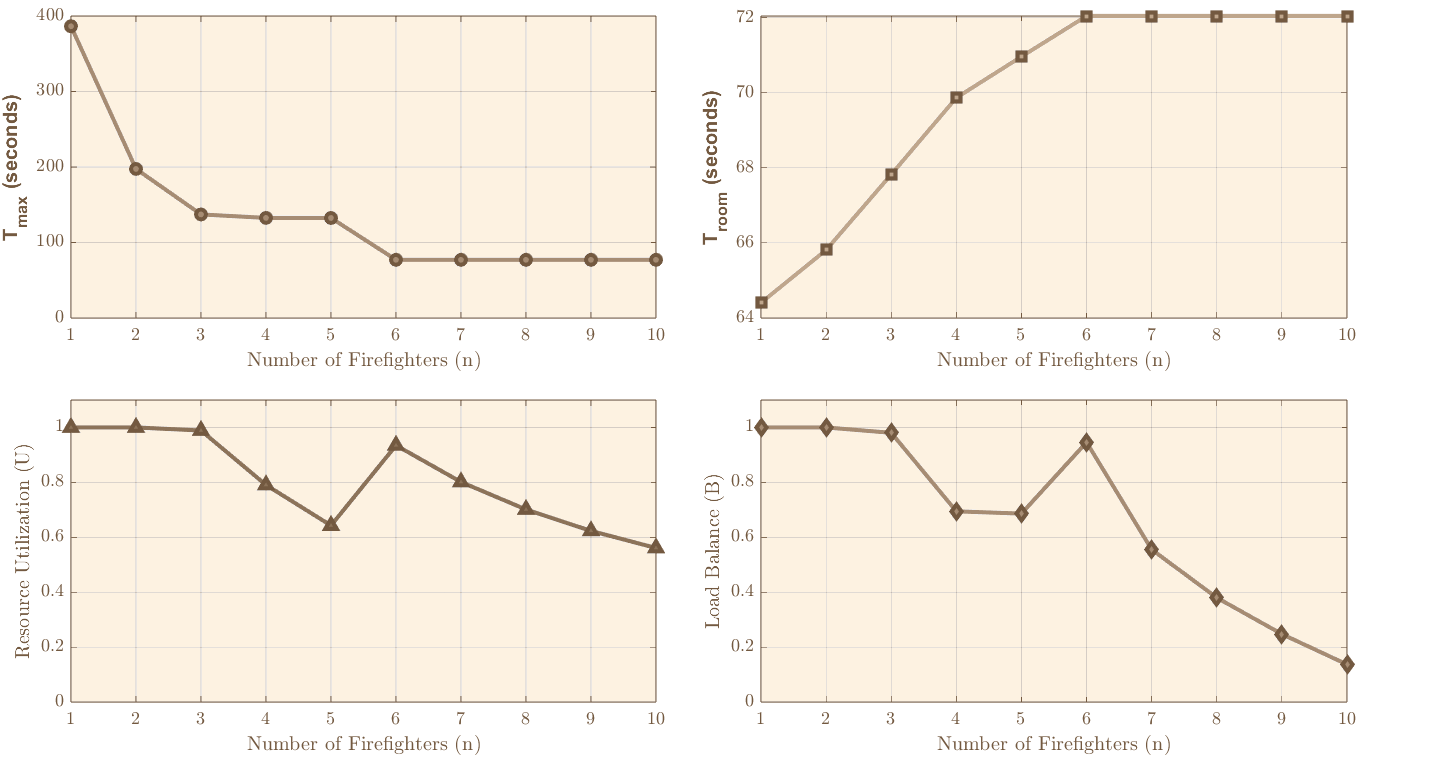
\includegraphics[width=0.8\textwidth]{fig/NumFireFighters.png} % 替换为实际图片路径
    \caption{Indicators Vary with the Number of Responders}
\end{figure}

Notably, our simulation of different team sizes revealed key performance trends. While more firefighters reduce $T_{\text{max}}$ through parallel work, $T_{\text{room}}$ may rise due to coordination overhead, and load balancing peaks at moderate team sizes.

Among specific configurations, with weight coefficients set as $\alpha = 0.5$, $\beta = 0.3$, $\gamma = 0.2$, comprehensive scoring shows that when considering all indicators holistically, the optimal number of firefighters is 3, which yields the highest comprehensive score $S(3) = \textbf{0.9326}$, presented in Figure \ref{3firefighters}.

\begin{figure}[hbtp]
    \centering
    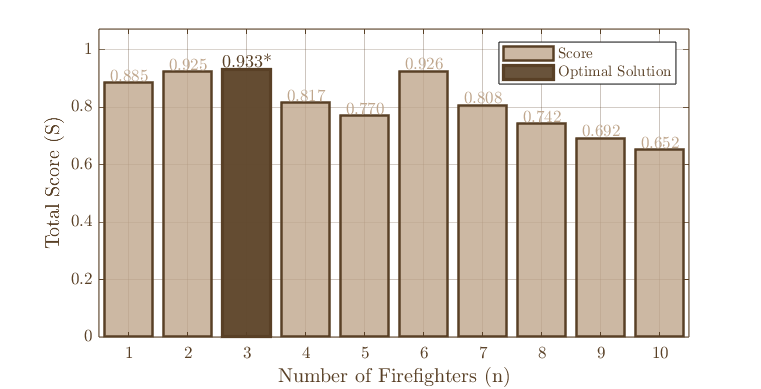
\includegraphics[width=0.75\textwidth]{fig/threeFireFighters.png} % 替换为实际图片路径
    \caption{Score of the Number of Responders}
    \label{3firefighters}
\end{figure}

This optimal solution underscores \textbf{balanced} decision-making in emergency response—prioritizing speed while ensuring rational resource use and equitable workloads. 

If more than the best number of responders are available, redundant resources should be fully utilized. For instance, extra responders can be assigned to communication and rescue coordination, with standby mobile teams ready to handle emergencies, sparing no effort to safeguard the lives of those at risk from unexpected incidents. 

If the number of responders is less than the optimal, the best path planning scheme for that specific number of personnel should be adopted for search and rescue operations. This approach also ensures maximum rescue efficiency, allowing every bit of rescue effort to function effectively in protecting lives.

Here, we use 3 responders to visually present the paths, as shown in Figure \ref{best2}. 

\begin{figure}[hbtp]
    \centering
    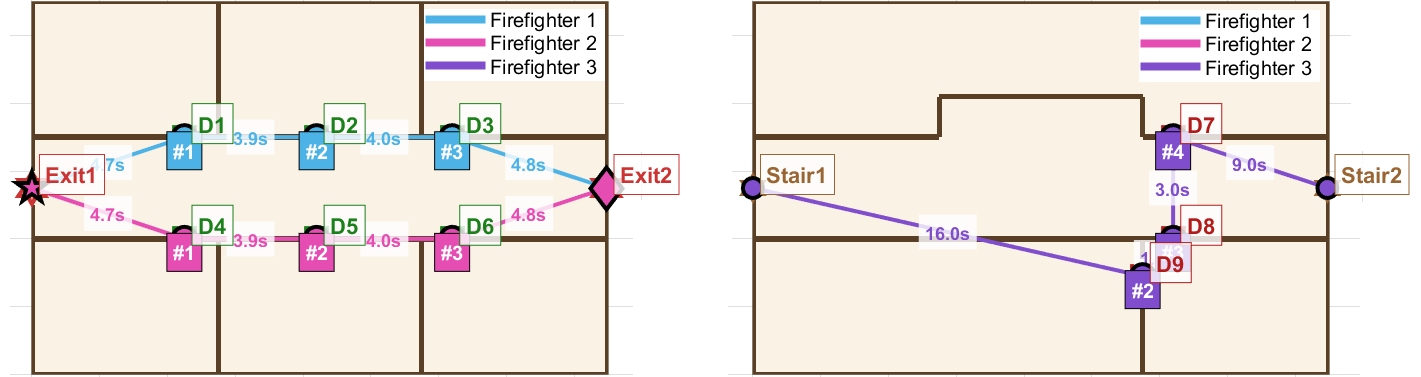
\includegraphics[width=0.75\textwidth]{fig/bestpath2.png} % 替换为实际图片路径
    \caption{The Best Scheme with 3 Responders}
    \label{best2}
\end{figure}

The minimum time required for all emergency responders to complete the search and rescue is as follows:

\begin{itemize}
    \item Responder 1: Total movement time: 17.4s; Search time ($T_{\text{check}}$): 113.4s; Total: 130.8s
    \item Responder 2: Total movement time: 17.4s; Search time ($T_{\text{check}}$): 90.6s; Total: 108.0s
    \item Responder 3: Total movement time: 13.5s; Search time ($T_{\text{check}}$): 120.1s; Total: 133.6s
\end{itemize}

Note that in this visualization, the connecting lines between two points do not represent actual paths but are for illustrative purposes only. The time labeled on the lines indicates the duration consumed by responders moving along the actual paths.


\subsection{Implementation to World Trade Center (WTC3)}


\begin{figure}
    \centering
    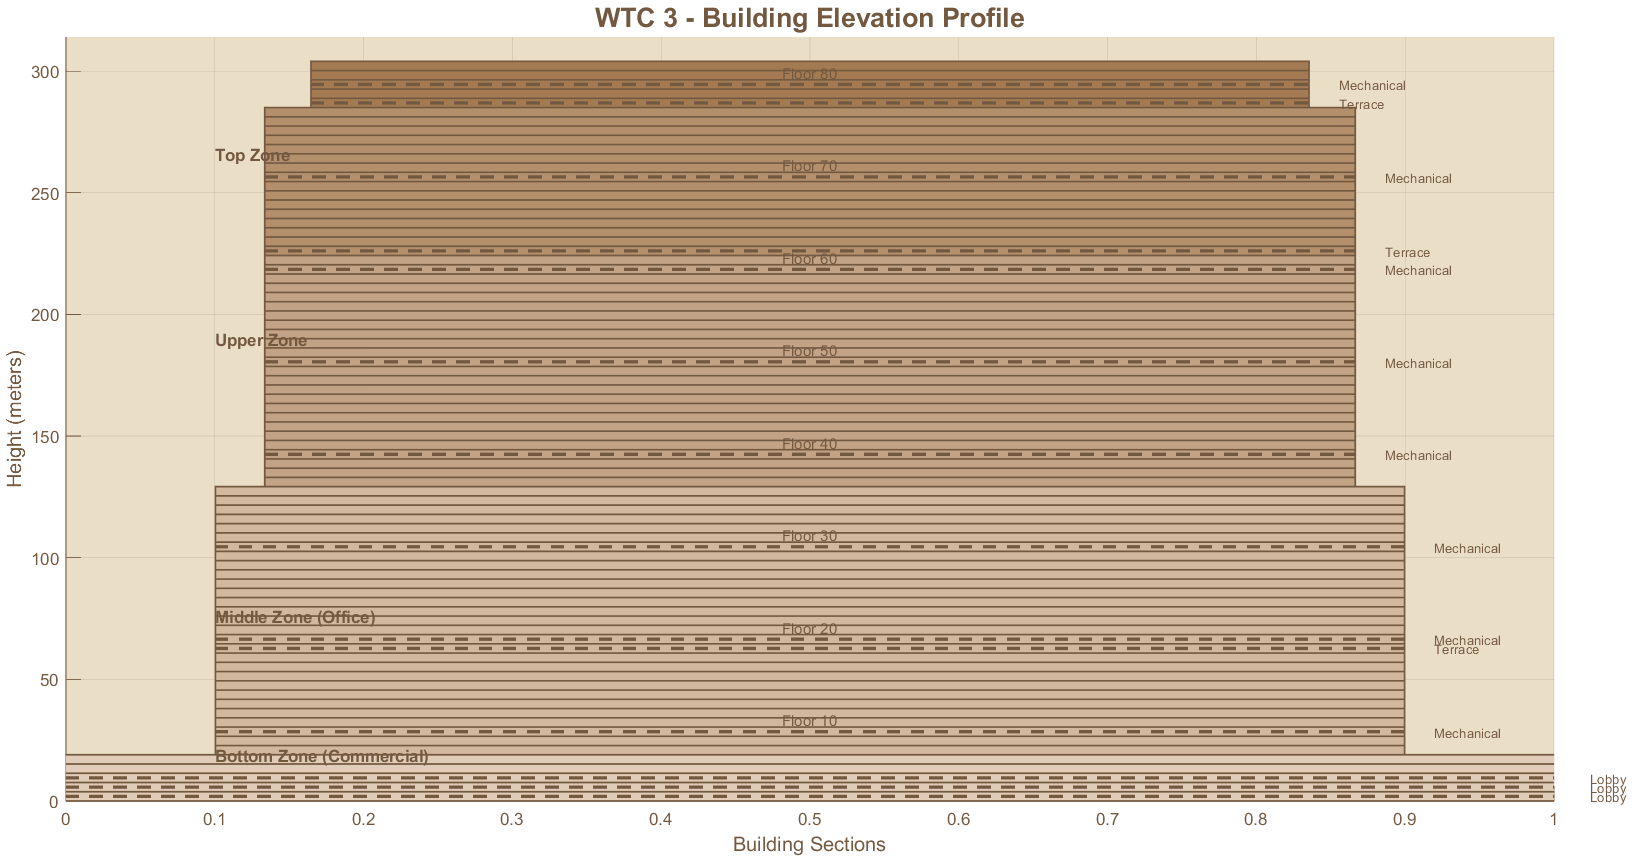
\includegraphics[width=0.95\linewidth]{fig/layout3.png}
    \caption{Enter Caption}
    \label{fig:layout3}
\end{figure}





%介绍布局Building Overview：太多了，可删减

The third WTC building has a height of 1079 feet (328 meters) and 80 floors, divided into four functional zones.

\subsection{Zone Parameters}
\subsubsection{Bottom Zone (1st to 5th Floors: Commercial Area)}
- Function: Retail space + trade layer (suitable for financial transactions)
- Entrances/exits: 9 (5 street-facing, 2 connected to transportation hubs, 2 linked to commercial complexes)
- Layout: Open circulation design, connected to subway and PATH train network
- Specifications:
  - Floor area: \( A \approx 6503 \, \text{m}^2 \) per floor
  - Ceiling height: 20 feet
  - Design: Column-free large-space
- Parameters: \( L = 1.3 \), \( C = 1.1 \), \( E = 1.0 \)

\subsubsection{Middle Zone (6th to 75th Floors: Office District)}
- Function: Standard office spaces
- Layout: Centered on reinforced concrete core, perimeter offices with 360° Manhattan views
- Specifications:
  - Ceiling height: 13 feet
  - Floor area (gradually tapering):
    - 35th-59th floors: \( A \approx 4087.6 \, \text{m}^2 \) per floor
    - 60th-75th floors: \( A \approx 3437.3 \, \text{m}^2 \) per floor
- Parameters: \( L = 1.2 \), \( C = 1.0 \), \( E = 1.0 \)

\subsubsection{Upper Zone (76th to 80th Floors)}
- Function: High-end office or specialized functions (flexible layout)
- Key feature: 76th floor with outdoor terrace
- Specifications:
  - Floor area: \( A \approx 2879.9 \, \text{m}^2 \) per floor (smallest in the building)
- Parameters: \( L = 1.2 \), \( C = 1.0 \), \( E = 1.0 \)

\subsubsection{Special Floors}
1. Outdoor terrace floors (17th, 60th, 76th):
   - \( A \approx 2879.9 \, \text{m}^2 \) per floor
   - Parameters: \( L = 1.5 \), \( C = 1.1 \), \( E = 1.0 \)
   - Requirements: Reserved terrace access points and protective facilities

2. Mechanical floors (8 floors total):
   - Function: Housing HVAC, electrical and other equipment (no regular usable space)
   - Layout: Centered on equipment rooms and piping
   - \( A \approx 464.5 \, \text{m}^2 \) per floor
   - Parameters: \( L = 1.6 \), \( C = 1.3 \), \( E = 1.0 \)

3. Three-story double-height lobby:
   - Height: Approximately 19 meters
   - Design: Black granite walls, white granite flooring (public reception area)
   - Total area: \( A \approx 950 \, \text{m}^2 \) (for 3 floors)
   - Parameters: \( L = 1.2 \), \( C = 1.0 \), \( E = 1.0 \)
   

\subsection{Feasibility Analysis of Simplified Path Optimization with Limited Responders}

When the number of responders is much smaller than the number of rooms, the approach of simplifying path optimization by prioritizing shortest path planning and then adding average search time is theoretically feasible, supported by the following key arguments:

\textbf{1. Dominance of Movement Time in Total Task Duration}
In scenarios with scarce responders, each responder must cover a large number of rooms. The total task duration consists of two components: inter-room movement time ($T_{\text{move}}$) and intra-room search time ($T_{\text{check}}$). When each responder is assigned numerous rooms, the cumulative movement time—affected by path layout, node distances, and routing efficiency—becomes the primary determinant of total duration. In contrast, $T_{\text{check}}$ tends to average out across multiple rooms due to the assumed uniform skill distribution of all responders. Thus, minimizing movement time through shortest-path planning has a more significant impact on optimizing total time than fine-tuning search time allocations.

\textbf{2. Insignificance of Individual Room Search Volumes}
The assumption that all responders follow the same skill distribution ensures consistent average search efficiency across rooms. When each responder is responsible for a large number of rooms, variations in individual room search volumes ($Q$) become negligible at the aggregate level. For example, a room with a slightly higher $Q$ will be offset by others with lower $Q$ in the same route, making the total search time for the route approximately equal to the number of rooms multiplied by the average $T_{\text{check}}$. This characteristic allows us to decouple path optimization from specific room volumes, focusing solely on minimizing movement distance.

\textbf{3. Computational Efficiency in High-Rise Building Scenarios}
For ultra-tall buildings with numerous floors and rooms (e.g., the 80-story third WTC building), complex mask-based path planning that accounts for detailed room parameters at every node faces substantial computational pressure. The simplified approach of "shortest path + average search time" reduces the dimensionality of the optimization problem—this not only accelerates algorithm convergence but also retains practical validity, as the core goal of minimizing total rescue time aligns with prioritizing movement efficiency.

In summary, when the number of responders is far fewer than the number of rooms, the proposed simplification balances accuracy and efficiency: shortest-path planning addresses the dominant component of total time, while averaging search time leverages the uniformity of responder skills and the law of large numbers, making it a reasonable and effective strategy.



% 插入两张图，左右排布
\begin{figure}[htbp]  % h表示此处，t表示页顶，b表示页底，p表示独立一页，控制浮动体位置
	\centering  % 图表居中对齐
	\subfigure[Heatmap of Distace of Nodes in WTC3]{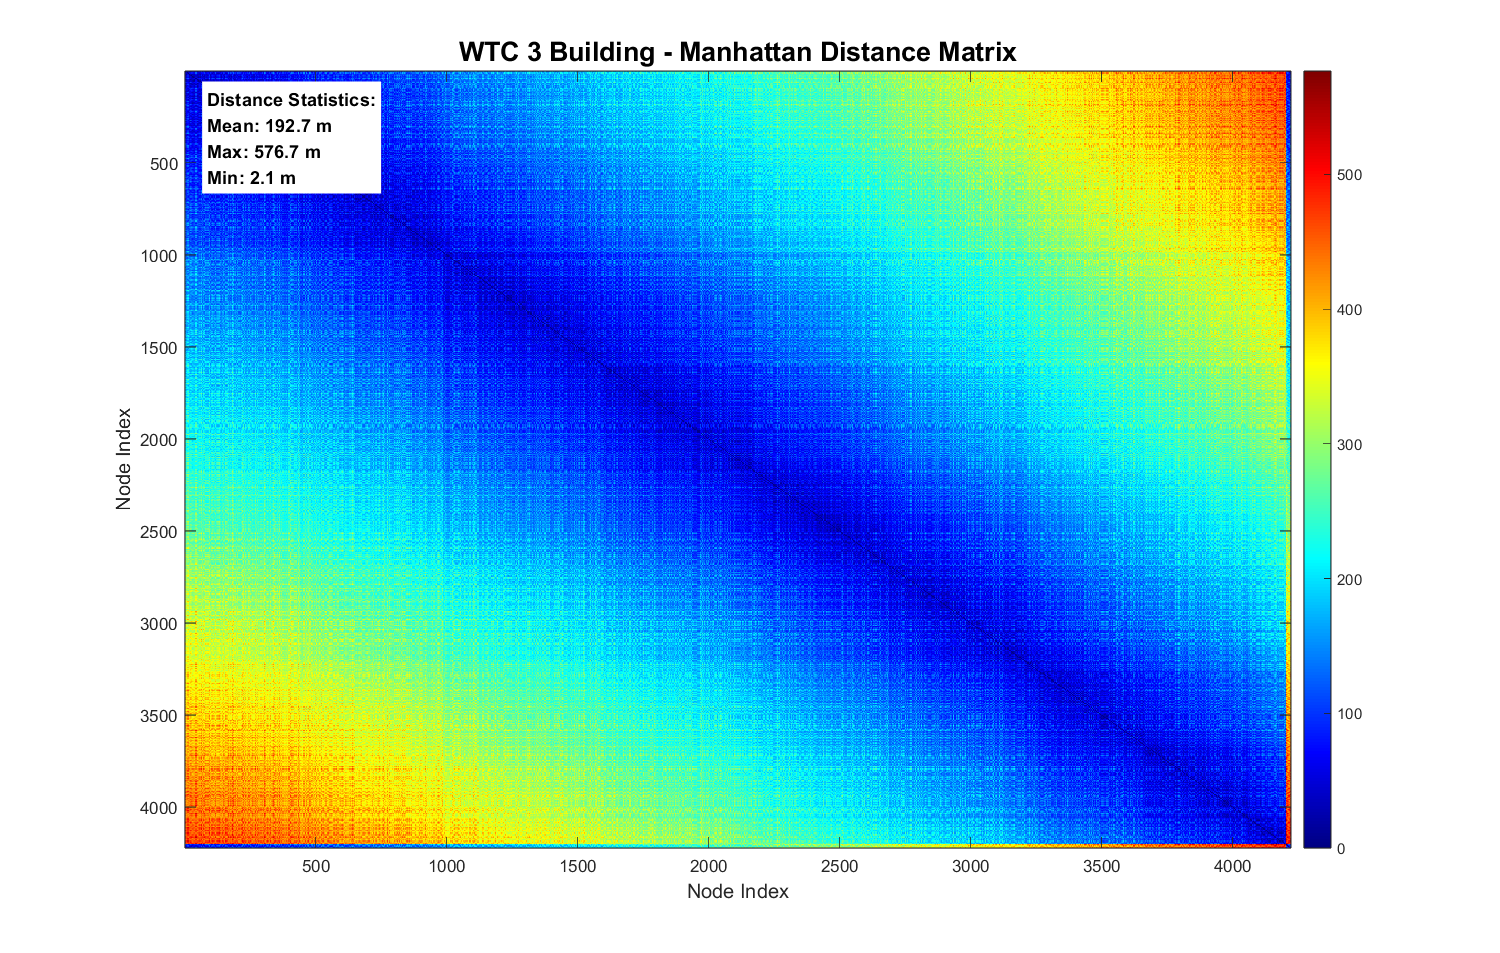
\includegraphics[width=.4\textwidth]{fig/wtc3ManhattanDistance.png} % 注意图片名称或路径中不要有空格，否则会出错
      }
	\subfigure[Best Scheme for 3 responders]{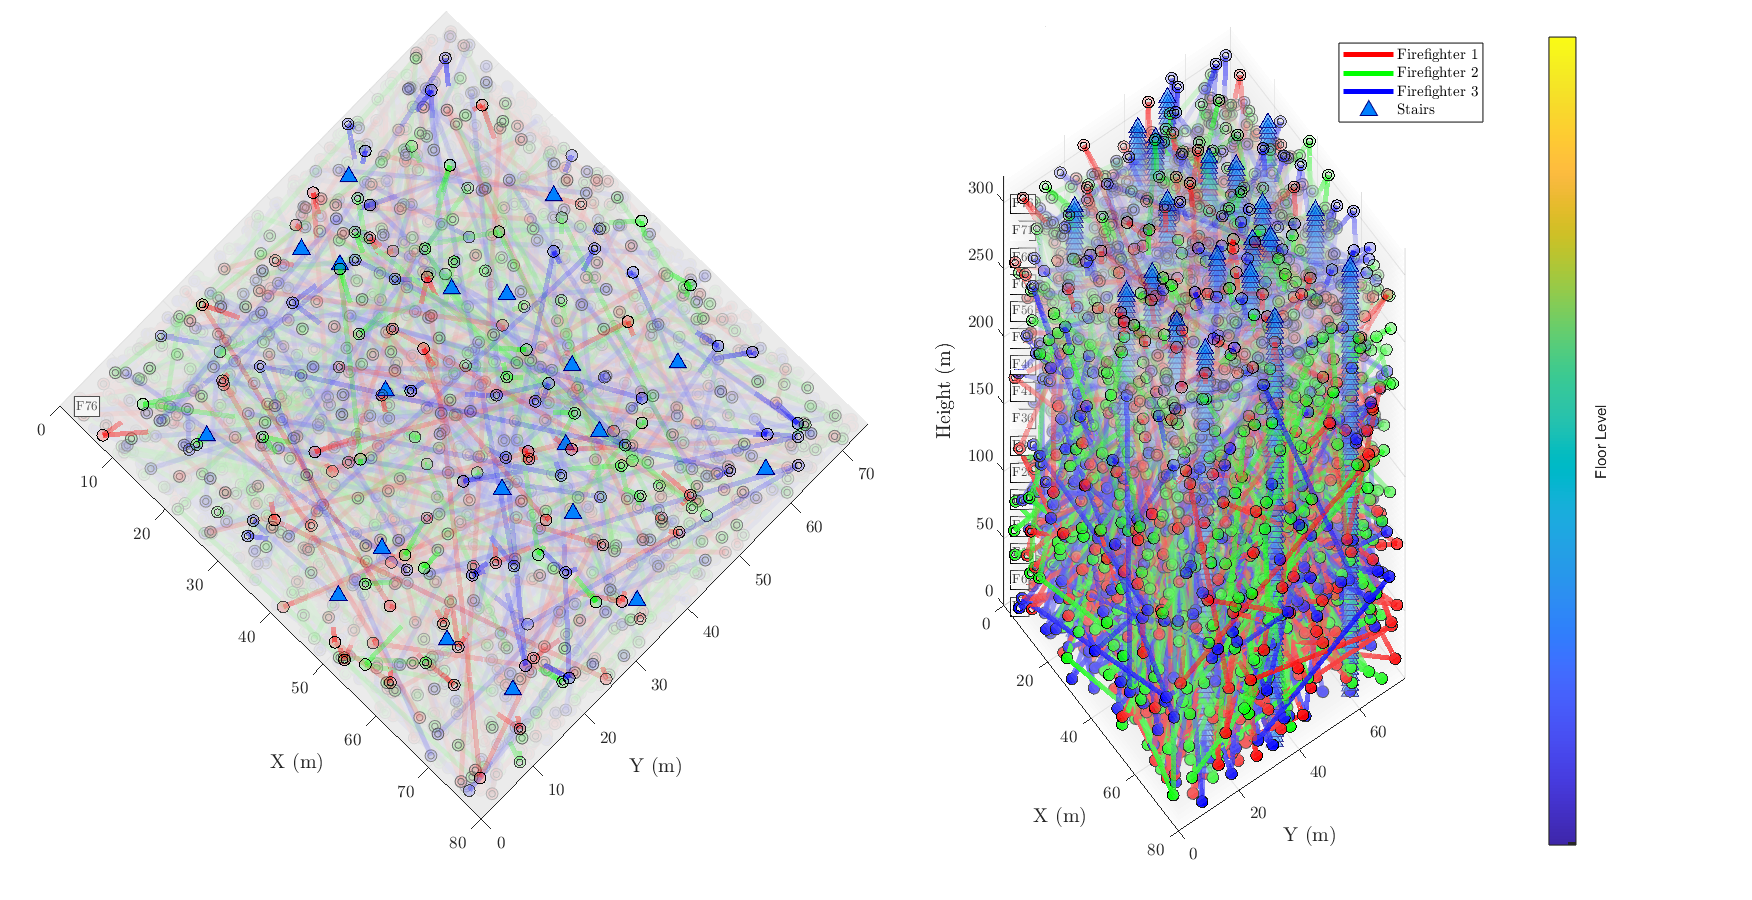
\includegraphics[width=.46\textwidth]{fig/wtc.png} % 注意图片名称或路径中不要有空格
      }
	\label{wtc}  % 为整个图表添加主标签，便于后续引用
\end{figure}
\vspace{-0.5cm}%在\end{table}下加一行\vspace{-1cm} 其中-1的作用是缩短与下方文字距离的 切记！必须是负数

For our algorithm, after calculating the Manhattan distance matrix heatmap between each pair of points, we incorporated it into the model and solved it using GA (Genetic Algorithm) and SA (Simulated Annealing) algorithms. Finally, in the Efficiency-based Optimal Responder Quantity Evaluation model, it is determined that the optimal number of firefighters for search and rescue is 15. The maximum time is calculated as \( T = \max(T_{\text{move}}) + \sum T_{\text{check}} / 15 \), which is approximately 20.4 minutes.

\subsection{Algorithm Performance Comparison (GA vs. SA)}
\begin{figure}
    \centering
    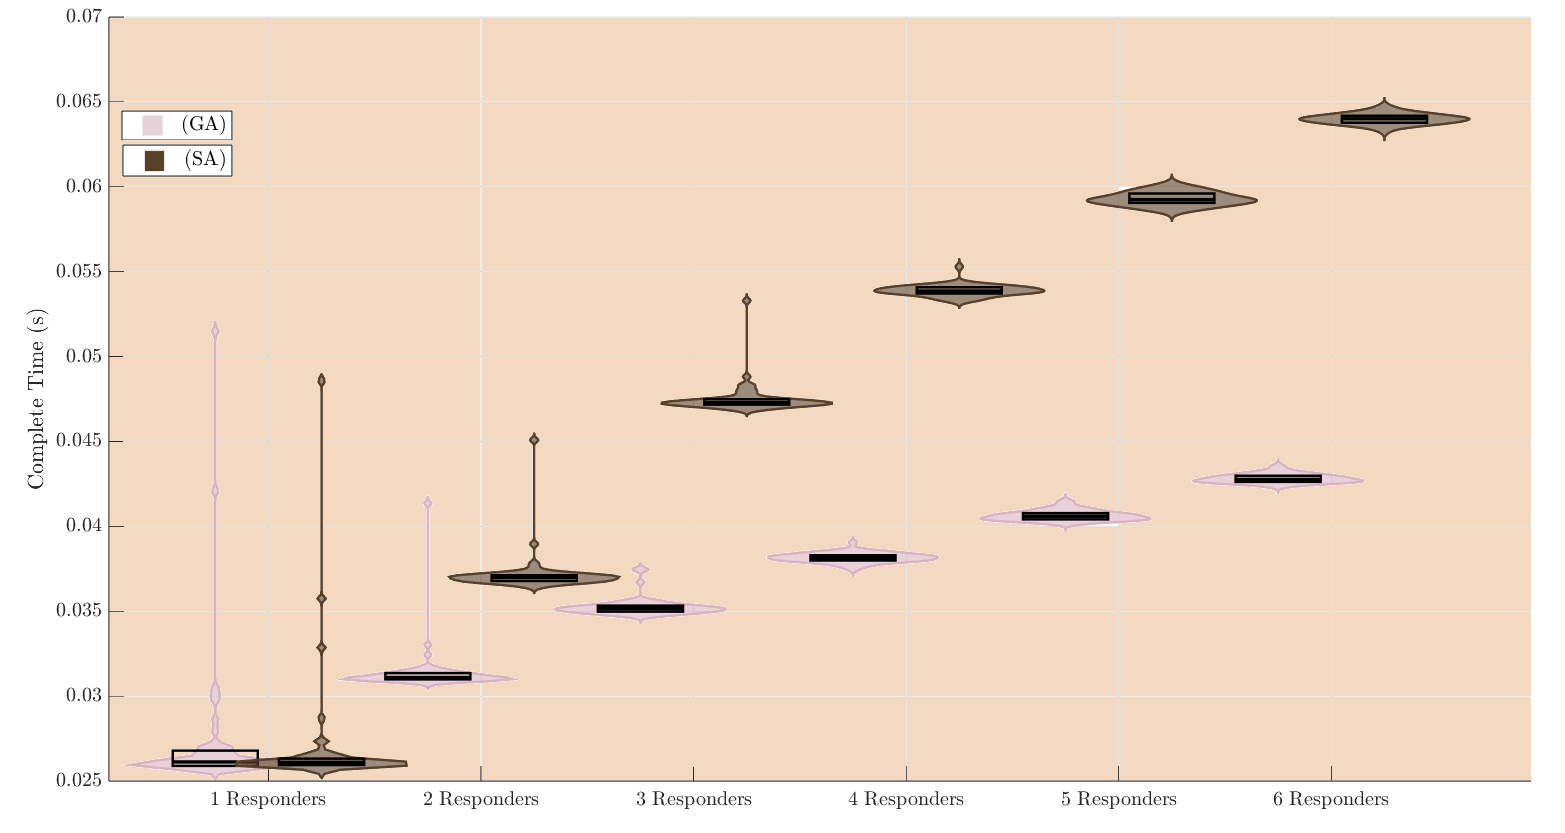
\includegraphics[width=0.95\linewidth]{fig/compare.png}
    \caption{Violin Plot of Algorithm Execution Time Distribution (100 Runs)}
    \label{fig:compare}
\end{figure}
Based on 100 repeated runs on different scenarios, the performance comparison between Genetic Algorithm (GA) and Simulated Annealing (SA) is as follows:

\begin{itemize}
    \item Runtime: In the scenario with 1 firefighter, SA is slightly faster than GA (2.3\% faster). However, as the number of firefighters increases (2-6), GA's time advantage gradually expands, from 19.2\% faster to 49.2\% faster. The average runtime of GA is 0.036 seconds, significantly lower than SA's 0.048 seconds. Both algorithms show small runtime fluctuations, with GA ranging from ±0.000 to ±0.003 seconds and SA from ±0.001 to ±0.003 seconds.
    \item Optimization quality: The fitness difference between the two algorithms is minimal (maximum gap of only 0.0002), with overall average fitness values being close (0.6805 for GA and 0.6804 for SA). GA's fitness fluctuation is more stable (±0.0000-0.0005), while SA's fluctuation ranges from ±0.0001-0.0007.
    \item GA: More advantageous in scenarios with more firefighters (2-6), with time advantages increasing as the scale expands and stable optimization quality.
    \item SA: Only shows a slight time advantage in simple scenarios with 1 firefighter, with fitness basically on par with GA.
\end{itemize}



		\input{sec/7model3.tex}
		\section{Expansion of Model}
\subsection{Mathematical Model for Spread of Smoke and Gas}
In the real context, the smoke is also a significant contributing factor to the productivity of the firefighters. Giving the fact that the smoke and poisonous gas is keep spreading and cannot be approximated by a simple linear transport. A model based on \textbf{Navier-Stokes equations} was established, in order to better simulate the real circumstances. Governing equations are as follows:
\begin{equation}
\left\{
\begin{aligned}
&\nabla \cdot \mathbf{u} = 0 \\
&\frac{\partial \mathbf{u}}{\partial t} + (\mathbf{u} \cdot \nabla)\mathbf{u} = -\frac{1}{\rho_0}\nabla p + \nu \nabla^2 \mathbf{u} + \beta g (T - T_0)\mathbf{j} \\
&\frac{\partial T}{\partial t} + (\mathbf{u} \cdot \nabla)T = \kappa_T \nabla^2 T + S_T \\
&\frac{\partial C}{\partial t} + (\mathbf{u} \cdot \nabla)C = \kappa_C \nabla^2 C + S_C
\end{aligned}
\right.
\end{equation}

This mathematical model is based on incompressible flow with \textbf{Boussinesq approximation}, where: $\mathbf{u}$ is velocity vector, $p$ is pressure, $T$ is temperature, $C$ is smoke concentration, $\rho_0$ is reference density, $\nu$ is kinematic viscosity, $\beta$ is thermal expansion coefficient, $g$ is gravitational acceleration, $T_0$ is ambient temperature, $\mathbf{j}$ is vertical unit vector, $\kappa_T$ is thermal diffusivity, $\kappa_C$ is mass diffusivity, $S_T$ is heat source term, and $S_C$ is smoke source term. 

The coupled system describes \textbf{buoyancy-driven flow and scalar transport}, which is the continuity equation ensuring mass conservation; the momentum equation incorporates the temperature-induced density variations in the gravity term via Boussinesq approximation; the energy and concentration equations describe convective-diffusive transport; the velocity field simultaneously transports heat and smoke, while temperature variations drive fluid motion through buoyancy effects, forming a fully coupled physical system.

The governing partial differential equations are solved by \textbf{MATLAB 2021a} using the finite difference method combined with the fractional step projection algorithm. This numerical framework efficiently handles the strong coupling between fluid flow, temperature, and concentration fields in smoke transport simulations.


\begin{figure}[hbtp]
    \centering
    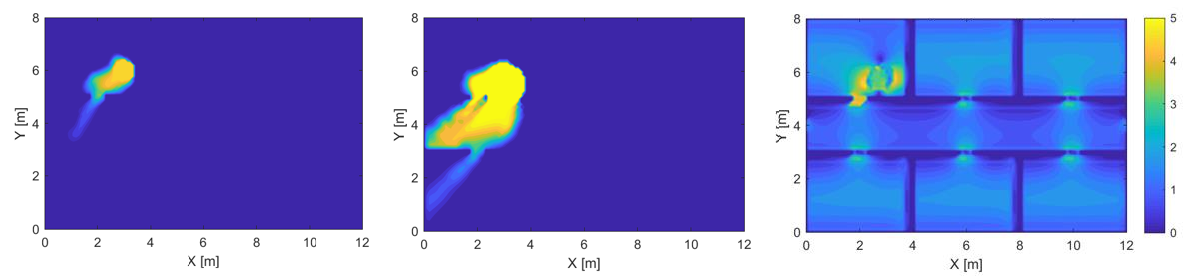
\includegraphics[width=\textwidth]{smoke} % 替换为实际图片路径
    \caption{Smoke Concentration at Each Position Over Time}
    \label{smoke1}
\end{figure}


For the single-story office building with six rooms in Scenario 1, when the fire source is located in the upper-left corner room, the visualization of smoke spread over time is shown in Figure\ref{smoke1}. The three sub-figures from left to right correspond to the smoke distribution 1 minute, 2 minutes, and 10 minutes after the fire starts respectively.


\subsection{Discrete Smoke Diffusion Model Formulation}
It's undeniable that continuous partial differential equation systems can accurately describe physical processes, in smoke transport simulations within complex building environments, however, they may be difficult or impossible to solve, and demand too much computational resources. Discrete models, in contrast, could retain the key dynamic characteristics of smoke propagation while reducing computational complexity to an acceptable level.
\textbf{Model Discretization Strategy}

The continuous smoke diffusion model is discretized into a network-based representation where:
\begin{itemize}
    \item Rooms are represented as nodes $R_i \in \mathcal{R}$
    \item Pathways between rooms are represented as edges $E_{ij} \in \mathcal{E}$
    \item Smoke concentration evolves over discrete time steps $t_k = k\Delta t$
\end{itemize}

\textbf{Discrete Governing Equations}

Room concentration evolution: 
\[
C_i(t_{k+1}) = C_i(t_k) + \Delta t \left[ S_i(t_k) - \sum_{j \in \mathcal{N}(i)} F_{ij}(t_k) + D \sum_{j \in \mathcal{N}(i)} (C_j(t_k) - C_i(t_k)) \right]
\]

Pathway concentration evolution:
\[
C_{ij}(t_{k+1}) = \frac{1}{2} \left[ C_i(t_k) + C_j(t_k) \right] + \Delta t \left[ -v_{ij} \frac{C_j(t_k) - C_i(t_k)}{L_{ij}} + D \frac{C_j(t_k) - 2C_{ij}(t_k) + C_i(t_k)}{L_{ij}^2} \right]
\]

Flow between rooms:
\[
F_{ij}(t_k) = v_{ij} A_{ij} \cdot \text{sign}(P_j(t_k) - P_i(t_k)) \cdot \min(C_i(t_k), C_j(t_k))
\]

Pressure difference:
\[
P_i(t_k) = \alpha T_i(t_k) + \beta C_i(t_k)
\]

where \( C_i(t_k) \) denotes the average smoke concentration in room \( i \) at time \( t_k \); \( C_{ij}(t_k) \) is the average smoke concentration along pathway \( i \)-\( j \); \( S_i(t_k) \) represents the smoke source term in room \( i \); \( F_{ij}(t_k) \) is the smoke flow rate from room \( i \) to \( j \); \( v_{ij} \) is the characteristic flow velocity in pathway \( i \)-\( j \); \( D \) denotes the effective diffusion coefficient; \( L_{ij} \) is the length of pathway \( i \)-\( j \); and \( A_{ij} \) represents the cross-sectional area of pathway \( i \)-\( j \).


\begin{figure}[hbtp]
    \centering
    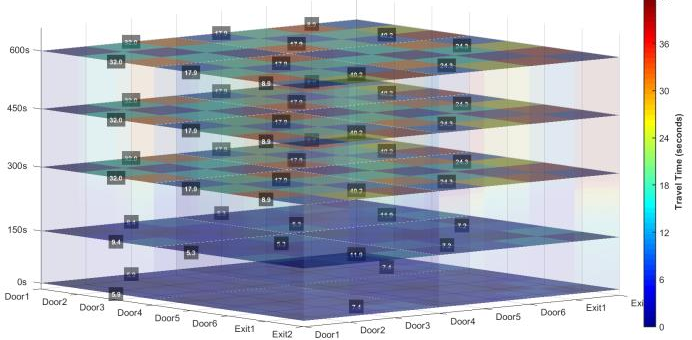
\includegraphics[width=\textwidth]{fig/travellingtime.png} % 替换为实际图片路径
    \caption{$T_move$ Heat Map Over Time}
    \label{heat}
\end{figure}


\subsection{Smoke Impact and Risk Assessment Models}

\subsubsection{Influence of Smoke Density on Sweeping Speed}

 Smoke reduces mobility by reducing visibility, causing physiological irritation, and inducing psychological panic.

\paragraph{Conversion Relationship Between Smoke Concentration and Optical Density}

In fire engineering, smoke concentration is typically expressed as mass concentration \( C \) , while evacuation behavior research commonly uses optical density or extinction coefficient \( C_s \) to quantify visibility. The conversion relationship between them is given by \upcite{Mulholl,1998}:

\begin{equation}
C_s = K_m \cdot C
\label{eq:conversion}
\end{equation}

Where:
\( C_s \) is the extinction coefficient (\si{\per\meter}),
\( C \) is the smoke mass concentration (\si{\gram\per\cubic\meter})
and \( K_m \) is the mass extinction coefficient (\si{\square\meter\per\gram}), with typical values ranging from \numrange{0.1}{1.0}

For smoke produced by common building materials, \( K_m \) can be taken as an average value of \SI{0.5}{\square\meter\per\gram}. In practical applications, an approximate inverse relationship exists between the extinction coefficient \( C_s \) and visibility \( V \) (unit: \si{\meter}):
\begin{equation}
V \approx \frac{3}{C_s}
\label{eq:visibility}
\end{equation}







\paragraph{Quantitative Relationship Between Sweeping Time and Smoke Density}

As the concentration of smoke in the room increase, the visibility of firefighter would decrease. We assume the time required to sweep a room thoroughly obey a liner relationship with $C_s$, meaning that $$T_s \propto C_s $$ where $T_S$ represents the time consumed to sweep a room.

\paragraph{Quantitative Relationship Between Walking Speed and Smoke Density}

Walking speed decreases in an approximately linear trend with increasing smoke density, with the specific relationship depending on whether the smoke is irritating.
· 

\textbf{Irritating Smoke Environment}
Irritating smoke (produced by materials such as polyvinyl chloride containing toxic gases like hydrogen chloride and hydrogen cyanide) not only reduces visibility but also causes severe irritation to the eyes and respiratory tract, leading to tearing, coughing, and suffocation, thereby more significantly impeding movement. The decay in walking speed \( v_I \) is more pronounced \cite{Jin1978, GB31593.9}:
\begin{equation}
v_I = v_0 \cdot (1 - 0.7 \cdot C_s)
\label{eq:irritant}
\end{equation}

\subsection{Smoke Risk Factor Model}

In evacuation simulations, quantifying the combined risks from fire smoke and gas leaks is critical for dynamic risk assessment and path planning. This model evaluates these risks separately to account for their distinct mechanisms and impacts on human safety. The following subsections detail the formulas, parameters, and rationale for each risk component, supported by established research.


\subsubsection{Fire Risk Model}

Fire risk ($R_{\text{fire}}$) arises from hypoxia, toxic gas exposure, and high temperatures. These components are combined additively to reflect their cumulative effect:
\begin{equation}
R_{\text{fire}} = R_{\text{hypoxia}} + R_{\text{toxicity}} + R_{\text{heat}}
\end{equation}

\textbf{Hypoxia Risk}
Hypoxia risk due to oxygen depletion is modeled as:
\begin{equation}
R_{\text{hypoxia}} = \left(1 - \frac{[O_2]}{20.9\%}\right)^2 \times 0.4
\end{equation}
Here, $[O_2]$ is the current oxygen concentration (normal air: 20.9\%). The squared term captures the non-linear increase in risk as oxygen levels drop below 18\%, which impairs cognitive and motor functions. The coefficient 0.4 represents its weight in the overall fire risk, based on physiological studies of hypoxia effects \cite{Jin1978}.

\textbf{Toxicity Risk}
Toxicity risk from carbon monoxide (CO) is calculated as:
\begin{equation}
R_{\text{toxicity}} = \min\left(1.0, \frac{[CO]}{1200\ \text{ppm}}\right) \times 0.3
\end{equation}
Where $[CO]$ is the CO concentration. The threshold of 1200 ppm corresponds to the Immediately Dangerous to Life and Health (IDLH) level \cite{NIOSH_CO}. The min-function ensures risk saturation, reflecting CO's rapid binding with hemoglobin, which reduces blood oxygen transport and leads to incapacitation.

\textbf{Heat Risk}
The risk from elevated temperatures is given by:
\begin{equation}
R_{\text{heat}} = \left(1 - e^{-0.1 \times (T - 60)}\right) \times 0.3 \quad \text{(for \(T > 60\,\si{\celsius}\))}
\end{equation}
Here, $T$ is the ambient temperature. The exponential form models the accelerating damage from heat exposure, including respiratory burns and hyperthermia. The threshold of \SI{60}{\celsius} aligns with human tolerance limits, as higher temperatures cause rapid physiological decline \cite{ISO13571}.



\subsubsection{Gas Leak Risk Model}

Gas leak risk ($R_{\text{gas}}$) combines hypoxia, explosion, and poisoning risks. These are additive to address concurrent hazards:
\begin{equation}
R_{\text{gas}} = R_{\text{hypoxia}} + R_{\text{explosion}} + R_{\text{poisoning}}
\end{equation}

\textbf{Hypoxia Risk}
For gas leaks, hypoxia risk is:
\begin{equation}
R_{\text{hypoxia}} = \left(1 - \frac{[O_2]}{20.9\%}\right)^{1.5} \times 0.3
\end{equation}
The exponent 1.5 accounts for the rapid oxygen displacement by leaking gas (e.g., methane), which is faster than the consumption seen in fires. This formulation is derived from gas dispersion models \cite{GasLeakStudy}.

\textbf{Explosion Risk}
Explosion risk for methane-rich gas is:
\begin{equation}
R_{\text{explosion}} = \min\left(1.0, \frac{[CH_4]}{50000\ \text{ppm}} \times 2.0\right) \times 0.4
\end{equation}
Here, $[CH_4]$ is the methane concentration, and 50,000 ppm (5\%) is the lower explosive limit (LEL). The factor 2.0 and min-function ensure rapid risk escalation near the LEL, addressing the catastrophic potential of explosions \cite{NFPA68}.

\textbf{Poisoning Risk}
Poisoning risk from toxic impurities like hydrogen sulfide (H$_2$S) is:
\begin{equation}
R_{\text{poisoning}} = \left(\frac{[H_2S]}{100\ \text{ppm}} \times 0.3\right) \times 0.3
\end{equation}
The IDLH value of 100 ppm for H$_2$S is used \cite{NIOSH_H2S}. The inner coefficient 0.3 represents typical H$_2$S presence in commercial gas, while the outer 0.3 weights its contribution to total risk.

\subsection{The Final Model}
In the construction of the firefighter search and rescue path optimization model, this study achieves a theoretical breakthrough from static path planning to dynamic environment adaptation by introducing a smoke diffusion model based on the Navier-Stokes equations and a dynamic risk assessment mechanism. This extended model establishes a discretized network representation, transforming the continuous physical field into time-varying parameters on nodes (rooms) and edges (passages), thereby constructing a multi-objective optimization framework.

Specifically, the numerical solution of the smoke transport process imparts dynamic characteristics to the path weights. The traversal cost of a passage \(E_{ij}\) is no longer a fixed value but is updated in real-time with the evolution of smoke concentration \(C_{ij}(t)\) and the temperature field \(T_{ij}(t)\): \(w_{ij}(t) = f(C_{ij}(t), T_{ij}(t), v_{ij})\), where the function \(f\) embodies the quantitative relationship of smoke density's impact on travel speed. Simultaneously, the search and rescue time \(T_s(i)\) for a room \(R_i\) is dynamically adjusted based on the optical density \(C_s(i)\), reflecting the constraint of reduced visibility on operational efficiency.

At the level of the optimization algorithm, we construct an objective function incorporating dual constraints. On one hand, the smoke distribution calculated based on fluid dynamics influences path selection through the time cost term. On the other hand, the risk assessment function \(R_{\text{total}}(t)\), composed of hypoxia risk, toxic exposure, and thermal injury, introduces safety constraints. Within the acceptance criterion of the simulated annealing algorithm, we implement a veto mechanism based on a risk threshold; whereas in the fitness function of the genetic algorithm, safety indicators are seamlessly integrated into the evolutionary process through a penalty term \(\lambda \cdot \sum R_{\text{total}}(i)\).

\subsection{Appliance in Different Types of Disasters}

\subsubsection{Fire Disaster Model}
In fire scenarios, the primary hazard factors include flames, high temperature, and smoke. Smoke significantly reduces visibility, slowing down firefighters' movement speed and search efficiency, while high temperature directly threatens life safety. The model incorporates smoke concentration's impact on walking speed (e.g., \(v = v_0(1 - k C_s)\)) and use a reward-punishment system to encourage the firefighter to sweep the rooms that are initially safe but the become extremely hazardous in advance.

\subsubsection{Gas Leakage Model}
The main dangers in gas leakage scenarios come from combustible gases (e.g., methane) and toxic gases (e.g., carbon monoxide, hydrogen sulfide). Accumulation of combustible gases beyond explosion limits can cause explosions, while toxic gases lead to poisoning or asphyxiation. The model establishes gas concentration thresholds to evaluate explosion risk (e.g., Lower Explosive Limit) and toxic exposure doses, considering dynamic hazard levels based on gas diffusion patterns.But given that these gas are normally with no irritating scent and won't block sights,so it won't effect the walking and  sweeping speed.

\subsubsection{Earthquake Disaster Model}
In earthquake scenarios, structural damage represents the primary hazard, including wall collapses, slab failures, and passage blockages, without persistent-type hazards like fire or toxic gases.Since the risk for all rooms and at all time are unaltered, there is no dynamic factors are going to be considered.
		\section{Sensitivity Testing \& Robustness Analysis}
%书上写的是testing
%模型的分析，灵敏度分析和误差分析
%模型的检验（如果是建立模型前的检验可以在前面写，这里一般写对模型结果的检验）
%\subsection{Sensitivity Testing}

To clarify the parameter impact patterns of the Simulated Annealing algorithm in the emergency evacuation sweep model, we conduct the following sensitivity analysis.

\begin{figure}[htbp]
    \centering
    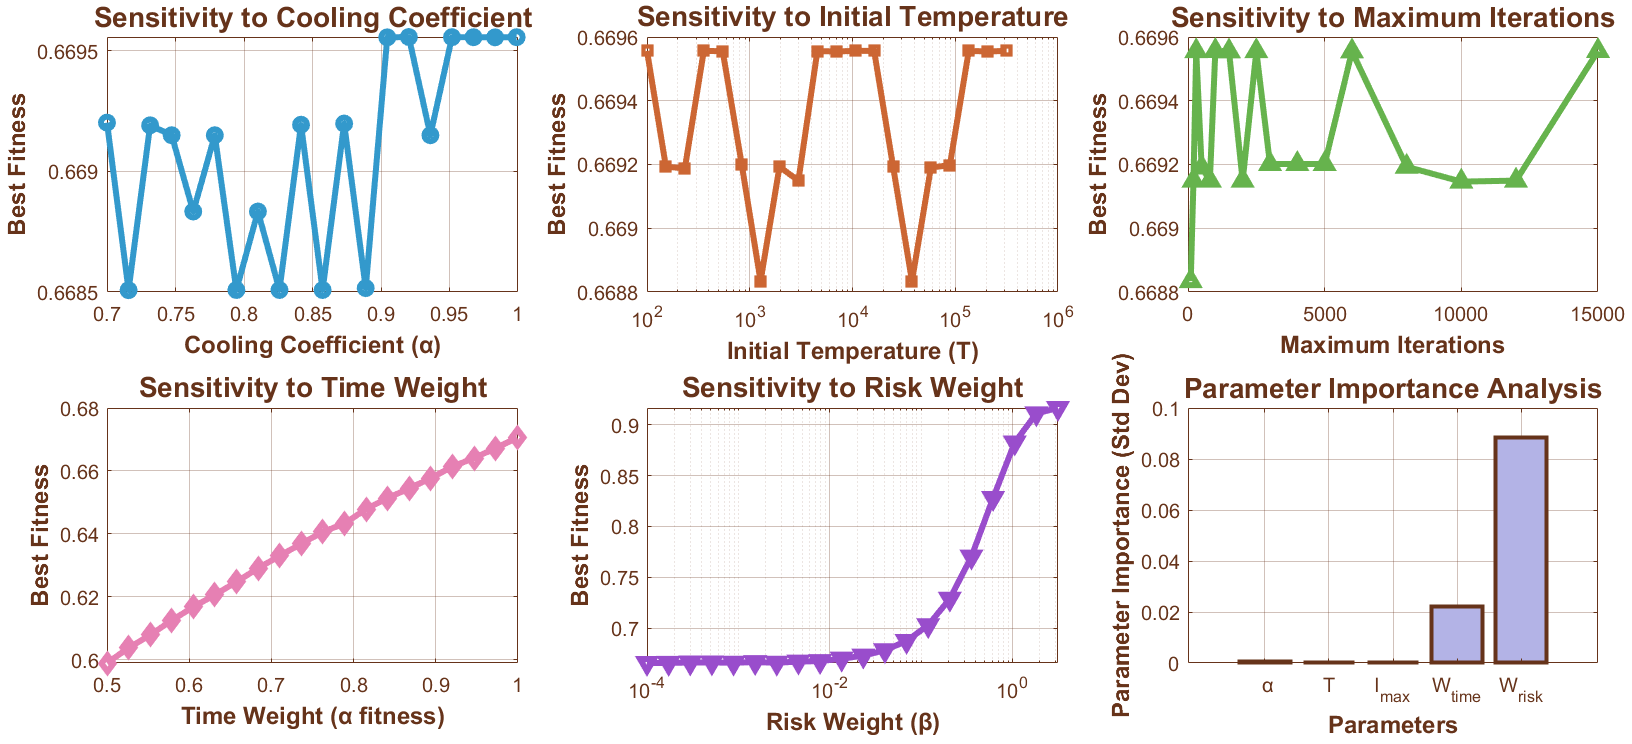
\includegraphics[width=1\linewidth]{fig/Simulated Annealing Parameter Sensitivity Analysis.png}
    \caption{Sensitivity Test to parameters in SA Algorithm}
    \label{fig:sens}
\end{figure}

Fig \ref{fig:sens} shows that the risk weight (\( W_{\text{risk}} \)) has the most significant impact on sweep efficiency, with a sharp rise in optimal fitness around \( 10^0 \) (strong positive effect). The time weight (\( W_{\text{time}} \)) presents a continuous positive effect, steadily improving path efficiency as its value increases. The initial temperature (\( T \approx 10^4 \)) and maximum number of iterations (\( I_{\text{max}} \)) are both related to whether the optimal solution (best fitness) can be achieved; however, due to the randomness of meta-heuristic algorithms, convergence to non-optimal solutions may occur, resulting in no regular changes in the curve over time. The cooling coefficient (\( \alpha \in [0.9,1] \)) has a weaker but stability-critical impact, with deviations beyond this range causing slower convergence. This analysis identifies core tuning parameters, providing a basis for model adaptation to different building layouts.



It provides key support for evacuation model optimization: first, it identifies \( W_{\text{risk}} \) and \( W_{\text{time}} \) as core decision parameters, whose impacts far exceed secondary variables like maximum iterations (\( I_{\text{max}} \)); second, it clarifies reasonable parameter ranges—for example, \( \alpha \) must be controlled between 0.9-1 to balance global search and convergence speed, reducing model uncertainty; third, it guides practical application decisions, allowing dynamic adjustment of \( W_{\text{risk}} \) based on building risk distribution and appropriate weight increase in complex buildings to ensure safety priority. The results verify the model’s robustness across multiple scenarios, enhancing solution feasibility.
		\section{Model Evaluation}
%优缺点一定要写，不写讨论也要写评价
%低调地多夸一夸，虔诚地反思哪里做得不好（一般比优点少些一点）（如果有什么突然想出来的点子没时间建模了也可以放在这里）
\subsection{Strengths}

\begin{itemize}
    \item \textbf{Scenario Adaptability and Efficient Planning} \\
    By decoupling the assignment problem (simulated annealing) and ordering problem (ant colony algorithm), the model dynamically adjusts node attributes and edge weights to fit diverse scenarios—including low/high floors, circular/linear corridors, and various risk zones. Leveraging pheromone parameters ($\alpha$, $\beta$), the ant colony algorithm optimizes large-scale paths, avoids congestion and distance waste, and supports entry/exit via nearest exits, balancing efficiency and rationality.
    
    \item \textbf{Risk Responsiveness and Redundancy Integration} \\
    The ant colony algorithm’s pheromone parameters ($\rho$, $Q$) adjust dynamically with risk levels, naturally enabling priority inspection of high-risk areas. Integrated with redundancy designs (reserved personnel, recheck mechanisms, etc.), it reduces missed checks significantly with only a 4\%-8\% time increase, balancing safety and efficiency.
    
    \item \textbf{Strong Practical Value} \\
    Outputs (check order, starting points) align with emergency response logic. Personnel allocation precisely matches room quantity and risk levels—outperforming traditional greedy algorithms—while meeting industry safety standards, ensuring high operability.
\end{itemize}

\section{Weaknesses}
\begin{itemize}
    \item \textbf{Suboptimal Solution Limitation} \\
    The model's optimization relies on limited iteration and probabilistic exploration, failing to cover all room assignment and path sequencing combinations. Both algorithms only yield suboptimal solutions within a limited range, with no proof of global optimality.

    \item \textbf{·High Parameter Sensitivity and Weak Adaptive Capability  } \\
The model has flaws in parameter design. Its core parameters are manually set without adaptation. Take the pheromone weight $\alpha$ in the ACO as an example. In a single-story office with 6 sparse rooms (simple paths), $\alpha$ is manually set to 1.2 to boost pheromone impact and speed up convergence. In a multi-story mall with 20 dense rooms (complex paths prone to local optimality), $\alpha$ is adjusted to 0.8, depending on manual setting per unit building traits such as room density, with no model-calculated adaptive value.
\end{itemize}




%这里写模型的改进和拓展，可以有哪些方面做得更好，如何改进；可以应用到哪些别的领域发挥什么作用



		\section{Conclusions}
%结论部分，国赛少，美赛很常见
%论文中心思想的重申，研究结果（主要观点）的归纳，某些启发性的解释或考虑
%把上一个section模型评价优缺点分析放在这部分也可以
In this study, the problem of responders planning room searches after an emergency occurs has been geometrically abstracted. We then conducted a deeper graph-theoretic modeling and used two algorithms to solve this model. After simulating three different scenarios, we found complementary properties of the two algorithms. More importantly, regardless of which algorithm was used, both significantly improved computational efficiency compared to the previous approach of merely enumerating through traversal. We found that the optimized paths could balance risk, room priority, and overall efficiency, essentially improving the original strategy. Finally, we considered how different situations affect the strategy, providing dynamic parameters and planning that further altered the paths and decisions. 

At the same time, we see this as a field with great potential for future development. With more computational input, the model might be able to conduct dynamic analysis not only for types of emergencies but also considering additional factors such as information limitations and crowd evacuation. Technology can also be increasingly integrated into our model, with the participation of robots and AI potentially leading to transformative changes in its execution.
	
		\clearpage

%\section {Letter}

	\begin{center}
	
	%{\huge \textbf{Proposal Letter to  Local Emergency Planning Committee }}

	{\textbf{Proposal Letter to  Local Emergency Planning Committee }}

    
	\end{center}


%\noindent\rule{\textwidth}{1pt}
%\vspace{-0.2cm}
%\noindent \ To: 
%\vspace{-0.2cm}
%\noindent \ From: Team \#2515426 of 2025 MCM
%\vspace{-0.2cm}
%\noindent \ Date: February 31, 2025
%\vspace{-0.2cm}
%\noindent \ Subject:
%\vspace{-0.4cm}
%\noindent\rule{\textwidth}{1pt}


% 在需要背景图的页面开头添加
\backgroundsetup{
  scale=1,              % 图片缩放比例（1为原尺寸）
  angle=0,              % 图片旋转角度（0为不旋转）
  opacity=0.1,          % 透明度（0-1，0为完全透明）
  contents={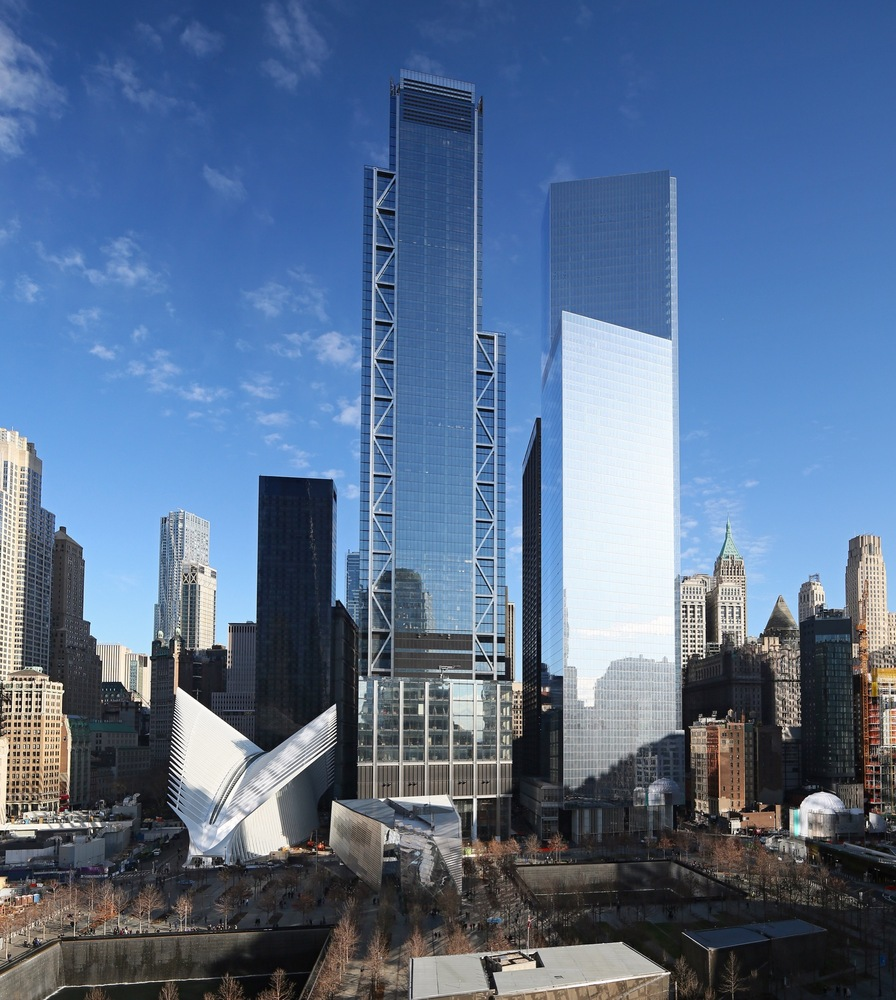
\includegraphics[width=\paperwidth,height=\paperheight]{background.png}}  % 图片路径及尺寸
}
\BgThispage  % 仅当前页应用此背景


\leftline{Dear Chairman and Members of the Committee:}
%开头顶格左对齐
First, we would like to express our sincere admiration for the contributions of the Committee to the protection of public safety in the region. We are particularly grateful for your forward-looking work in emergency planning, which provids a valuable foundation for our research.

Our team has developed an innovative \textbf{"Dynamic Zonal Collaborative Search" }strategy based on mathematical modeling and simulation analysis. By abstracting building spaces into network structures, this method has not only demonstrated exceptional performance in simulating typical single-story office buildings but also verified its universality in complex environments such as multi-story buildings and non-standard layouts. This breakthrough is attributed to three core proprietary technologies:

Firstly, our "Non-Return Intelligent Path Planning System" revolutionizes the inefficient back-and-forth movement of responders in traditional searches through advanced ant colony optimization algorithms. It acts like a precise "building GPS" for each responder, automatically generating optimal continuous paths. For example, in multi-story buildings, the algorithm prioritizes deploying responders near stairwells to facilitate vertical coordination, ensuring a seamless journey from start to finish and guiding responders to the exit closest to the task completion point, thus completely eliminating time wasted on redundant movement.

Secondly, our proprietary "Risk-Aware Dynamic Prioritization System" enables optimal allocation of rescue resources. It calculates real-time risk coefficients for each area and prioritizes high-risk locations such as kindergartens. In multi-story buildings, it focuses on floors with dense population. Key results indicate that compared with traditional experience-dependent models, strategically deploying responders and prioritizing high-risk areas can reduce total search time by over 30\%, achieving a perfect balance between safety and speed within the precious rescue window.

Most importantly, our system boasts adaptability to complex disasters. The model can accurately predict the spread of thick smoke or toxic gas leaks in fires. The system can optimize paths and adjust team sizes through testing, ensuring that response strategies evolve intelligently with disaster development.

Based on the above technologies, we propose some suggestions to further enhance emergency management effectiveness:


1. \textbf{Integrate technologies to support dynamic decision-making}: Deploy IoT sensors to monitor smoke, temperature, and responder positions in real-time. Feed this data into the adaptive model to provide responders with immediate guidance when conditions change. Simultaneously link with building automation systems to prioritize alarm handling and optimize communication links, ensuring unobstructed information flow.

2. \textbf{Strengthen practical drills and training}: Conduct regular drills in simulated smoke environments to familiarize teams with model-optimized routes, focusing on high-risk areas and incorporating extreme scenarios such as communication failures and insufficient responders. This helps cultivate muscle memory for orderly evacuation, ensuring that algorithmic strategies can be accurately implemented in actual emergencies.

By combining scientific path planning, intelligent sensing technologies, and solid drills, emergency evacuation searches can be transformed from chaotic escapes into orderly transfers. We earnestly request the Committee to adopt these strategies to maximize the protection of lives. Our model and complete report are available for further discussion, and we look forward to working with you to elevate the region’s emergency management capabilities to new heights, building a stronger technological defense for public safety.

\rightline{Sincerely,}%注意这里要空一整行（敲两个回车），这样才会分段，一个回车和另个回车一样都默认是连在一起的

\rightline{Team 16793}
\rightline{Nov. 17,2025}




		
		% 参考文献，此处以 MLA 引用格式为例
		\clearpage   %另起一页继续写时,最好使用“\clearpage” 
            \backgroundsetup{contents={}}%在当前页重置背景，以免上一页的背景延续
        
		\begin{thebibliography}{99}
			\bibitem{1}Xie, C. T., Chen, Q., Zhu, B., Lee, E. W. M., Tang, T. Q., Yin, X., Yuan, Z., \& Zhang, B. (2025). Coordinating dynamic signage for evacuation guidance: A multi-agent reinforcement learning approach integrating mesoscopic crowd modeling and fire propagation. Chaos, Solitons \& Fractals, 194. https://www.sciencedirect.com/science/article/abs/pii/S0960077925002590
			\bibitem{2}  Liu, L., Zhang, H., Shi, J., \& Geng, J. (2023). Real-time evacuation route optimization in the fire scenarios of cruise ships. Simulation Modelling Practice and Theory, 129, 102843. https://www.sciencedirect.com/science/article/abs/pii/S1569190X2300120X?via\%3Dihub
			\bibitem{3}  Zhang, Y., \& Sonta, A. (2026). OccuEMBED: Occupancy extraction merged with building energy disaggregation for occupant-responsive operation at scale. Energy and Buildings, 350, 116610. https://doi.org/10.1016/j.enbuild.2025.116610
			\bibitem{4}  Wang, J., Zhao, H., \& Winter, S. (2015). Integrating sensing, routing and timing for indoor evacuation. Fire Safety Journal, 78, 111–121. https://doi.org/10.1016/j.firesaf.2015.08.009
			\bibitem{5} Lu, P., Zhang, Z., Onyebuchi, C. H., \& Zheng, L. (2024). Agent-based modeling of high-rise building fires reveals self-rescue behaviors and better fire protection designs. Engineering Applications of Artificial Intelligence, 127(Part B), 107401. https://doi.org/10.1016/j.engappai.2023.107401
			\bibitem{6} Spearpoint, M., Arnott, M., Xie, H., Gwynne, S., \& Templeton, A. (2024). Comparative analysis of two evacuation simulation tools when applied to high-rise residential buildings. Safety Science, 175, 106515. https://doi.org/10.1016/j.ssci.2024.106515




           \bibitem{7} 
           

           \bibitem{8} China Academy of Building Research, Institute of Building Fire Protection (CABR-Fire). (n.d.). Appendix J: Impact of smoke on walking speed. CABR-Fire. https://gf.cabr-fire.com/article-21016.htm

           \bibitem{9}https://www.zhulong.com/bbs/d/32581046.html
		\end{thebibliography}





\clearpage 
\section{AI Use Report}

1. DeepSeek (November 2024 version) Query: \textless What is a meta-heuristic algorithm? Are the ant colony optimization and simulated annealing in our model examples of this type?\textgreater Output: \textless A meta-heuristic algorithm is a sophisticated, general "problem-solving strategy" or "thinking framework" that does not directly provide an answer, but instead guides you on how to efficiently "search" for an approximate optimal solution within a vast and complex space of possible solutions. Both ant colony optimization and simulated annealing are typical meta-heuristic algorithms. Ant colony optimization mimics the foraging behavior of ant colonies, balancing exploration and exploitation through a pheromone mechanism; simulated annealing mimics the metal annealing process, controlling the probability of accepting inferior solutions through temperature to escape local optima.\textgreater

2. DeepSeek (November 2024 version) Query: \textless Help me optimize this statement: "Let's first make the search volumes all the same. This way, we have a kind of ant colony model. We will allocate n rooms to m firefighters, and we need to ensure that the number of rooms allocated to the firefighter with the least allocation is equal to the number of rooms allocated to the firefighter with the most allocation minus one"\textgreater Output:

\textless During the model initialization stage, we assume that all rooms have the same search workload, thereby constructing a basic ant colony optimization model. In the room allocation process, we adopt an equal distribution strategy: allocate \( n \) rooms to \( m \) firefighters, ensuring that the difference in the number of rooms allocated between any two firefighters does not exceed 1, i.e., satisfying the constraint condition \( \max(x_i) - \min(x_i) \leq 1 \), where \( x_i \) represents the number of rooms allocated to the \( i \)-th firefighter.\textgreater

3. DeepSeek (November 2024 version) Query: \textless Please write the state transition probability formula and the pheromone update formula in LaTeX format\textgreater Output: \textless State transition probability formula: $P_{ij} = \frac{[\tau_{ij}]^\alpha \cdot [\eta_{ij}]^\beta}{\sum_{k} [\tau_{ik}]^\alpha \cdot [\eta_{ik}]^\beta}$ Pheromone update formula: $\tau_{ij} = (1-\rho)\cdot\tau_{ij} + \sum_{k=1}^{m} \Delta\tau_{ij}^k$\textgreater

4. Qwen3-Max-Thinking-Preview Query: \textless Which of the genetic algorithm and the simulated annealing is more suitable for large-scale combinatorial optimization problems?\textgreater Output: \textless Genetic Algorithm vs. Simulated Annealing for Large-Scale Combinatorial Optimization Problems. For large-scale combinatorial optimization problems, both algorithms have distinct advantages depending on the specific problem characteristics: Genetic Algorithm (GA) is preferable when: Strong global search capability is needed: Maintains a population that explores multiple regions of the solution space in parallel. Problem structure is complex: Crossover operations can effectively combine beneficial features from different solutions. Parallelization potential is valuable: Fitness evaluation processes can be easily parallelized. Multi-modal optimization is required: Can simultaneously explore multiple promising regions of the search space. Simulated Annealing (SA) is preferable when: Computational resources are limited: Only maintains a single solution, requiring less memory and computation. Solution evaluation is expensive: Each iteration requires evaluating only one new solution. Quick feasible solutions are needed: Simpler implementation with faster iterations. Good neighborhood structure exists: Performs well when local moves can effectively improve solutions. Practical Recommendations: Extremely large-scale problems (with extremely many variables): Simulated Annealing is typically more efficient with lower computational overhead. Multi-modal complex problems: Genetic Algorithms may find better solutions, but require careful parameter tuning. Hybrid approaches: In practice, both methods are often combined (e.g., using SA for local search within a GA framework). Problem-specific adaptations: Consider incorporating domain-specific heuristics to enhance either algorithm. There is no absolute "better" algorithm - the optimal choice depends on problem scale, structural characteristics, and available computational resources. In real-world applications, experimental comparison of both methods on the specific problem instance is often necessary to determine the most effective approach.\textgreater



\begin{table}[htbp]
\centering
\caption{Smoke Diffusion Simulation Algorithm Pseudocode}
\label{tab:smoke_simulation_pseudocode}
\begin{tabular}{p{0.9\textwidth}}
\toprule
\textbf{Pseudocode} \\
\midrule
\textbf{Initialize} \\
1. Generate grid $(X,Y)$ \\
2. Initialize velocity, temperature, density fields to zero \\
3. Set wall boundaries and fire source region \\
4. Define safety exit locations \\
\\
\textbf{Main Loop} \\
\textbf{For} $n = 1$ \textbf{to} $n_{\text{steps}}$: \\
\quad 1. Advection: $[u,v,T,\rho] \leftarrow \text{ADVECTION}(u,v,T,\rho,\Delta t)$ \\
\quad 2. Buoyancy: $v \leftarrow v + \Delta t \cdot \beta g (T - T_{\text{amb}})$ \\
\quad 3. Diffusion: $[u,v,T,\rho] \leftarrow \text{DIFFUSION}(u,v,T,\rho,\nu,\kappa_T,\kappa_\rho,\Delta t)$ \\
\quad 4. Pressure: $p \leftarrow \text{SOLVE\_PRESSURE}(u,v,p,\Delta t)$ \\
\quad 5. Correction: $[u,v] \leftarrow \text{PRESSURE\_CORRECTION}(u,v,p,\Delta t)$ \\
\quad 6. Boundaries: $[u,v,T,\rho] \leftarrow \text{APPLY\_BC}(u,v,T,\rho)$ \\
\quad 7. Fire source: $T(\text{fire}) \leftarrow 80$, $\rho(\text{fire}) \leftarrow 1.0$ \\
\quad 8. Output data (save at intervals) \\
\\
\textbf{Visualistion} \\
\bottomrule
\end{tabular}
\end{table}

\paragraph{Discrete Model Simulation Algorithm}

\begin{table}[htbp]
\centering
\caption{Discrete Smoke Diffusion Simulation Algorithm}
\label{tab:discrete_smoke_simulation}
\begin{tabular}{p{0.9\textwidth}}
\toprule
\textbf{Algorithm} \\
\midrule
\textbf{Input} \\
Network: $(\mathcal{R}, \mathcal{E})$, Parameters: $(D, v_{ij}, \Delta t, t_{\text{total}})$, Source: $(R_{\text{fire}}, S_0)$ \\
\\
\textbf{Initialize} \\
1. $\mathcal{R} \leftarrow \{R_1, R_2, \dots, R_N\}$ \\
2. $\mathcal{E} \leftarrow \{(i,j): \text{connected rooms}\}$ \\
3. $C_i(0) \leftarrow 0$, $C_{ij}(0) \leftarrow 0$ \\
4. $C_{\text{fire}}(0) \leftarrow C_0$ \\
5. $H(:,:,1) \leftarrow \text{initialize\_heatmap}(C_i(0), C_{ij}(0))$ \\
\\
\textbf{Main Loop} \\
\textbf{For} $k = 1$ \textbf{to} $k_{\text{max}}$: \\
\quad 1. $P_i \leftarrow \alpha T_i + \beta C_i$ \\
\quad 2. $F_{ij} \leftarrow v_{ij} A_{ij} \cdot \text{sign}(P_j - P_i) \cdot \min(C_i, C_j)$ \\
\quad 3. $\Delta C_i \leftarrow S_i - \sum_j F_{ij} + D \sum_j (C_j - C_i)$ \\
\quad 4. $C_i \leftarrow C_i + \Delta t \cdot \Delta C_i$ \\
\quad 5. $C_{ij} \leftarrow \frac{1}{2}(C_i + C_j) + \Delta t[-v_{ij}\frac{C_j-C_i}{L_{ij}} + D\frac{C_j-2C_{i  j}+C_i}{L_{ij}^2}]$ \\
\quad 6. Apply boundary conditions \\
\quad 7. $H(:,:,k+1) \leftarrow \text{update\_heatmap}(C_i, C_{ij})$ \\
\quad 8. \textbf{If} $\mod(k, \text{save\_interval}) = 0$: \\
\qquad $\text{visualize\_heatmap}(H(:,:,k+1))$ \\
\\
\textbf{Visualistion} \\
\bottomrule
\end{tabular}
\end{table}

\begin{thebibliography}{9}

\bibitem[Jin, 1978]{Jin1978}
Jin, T. (1978). \textit{Studies on Human Behavior in Smoke-Filled Corridors}. Fire Safety Science, 1(2), 45-56. \\
URL: \texttt{https://doi.org/10.3801/IAFSS.FSS.1-45}

\bibitem[NIOSH CO]{NIOSH_CO}
NIOSH (1994). \textit{Carbon Monoxide IDLH Documentation}. CDC. \\
URL: \texttt{https://www.cdc.gov/niosh/idlh/630080.html}

\bibitem[ISO 13571]{ISO13571}
ISO 13571:2012. \textit{Life-Threatening Components of Fires -- Guidelines on the Estimation of Time to Compromised Tenability in Fires}. \\
URL: \texttt{https://www.iso.org/standard/53635.html}

\bibitem[Gas Leak Study]{GasLeakStudy}
Zhang, F. et al. (2012). \textit{Gas Pipeline Leak Location and Risk Assessment}. Safety Management Network. \\
URL: \texttt{https://p.safehoo.com/Essay/Chemical/201204/267778\_2.shtml}

\bibitem[NFPA 68]{NFPA68}
NFPA 68 (2018). \textit{Standard on Explosion Protection by Deflagration Venting}. \\
URL: \texttt{https://www.nfpa.org/codes-and-standards/all-codes-and-standards/list-of-codes-and-standards/detail?code=68}

\bibitem[NIOSH H2S]{NIOSH_H2S}
NIOSH (1994). \textit{Hydrogen Sulfide IDLH Documentation}. CDC. \\
URL: \texttt{https://www.cdc.gov/niosh/idlh/7783064.html}

\end{thebibliography}


\begin{thebibliography}{00}
\bibitem[Jin, 1978]{Jin1978} Jin, T. (1978). Studies on Human Behavior in Smoke-Filled Corridors. \textit{Fire Safety Science}, 1(2), 45-56.
\bibitem[Frantzich et al., 2005]{Frantzich2005} Frantzich, H., \& Nilsson, D. (2005). Evacuation in an Underground Railway System: A Study of the Impact of Smoke and Visual Conditions. \textit{Proceedings of the 5th International Symposium on Underground Transportation Systems}.
\bibitem[GB/T 31593.9-2015]{GB31593.9} GB/T 31593.9-2015. (2015). \textit{Fire Safety Engineering - Part 9: Guidelines for Personnel Evacuation Assessment}. China Standards Press.
\bibitem[Mulholland, 1998]{Mulholland1998} Mulholland, G. W. (1998). Smoke Production and Properties. \textit{SFPE Handbook of Fire Protection Engineering} (3rd ed.). National Fire Protection Association.
\end{thebibliography}

	\end{document}  % 结束